\documentclass{cumcmthesis}
%\documentclass[withoutpreface,bwprint]{cumcmthesis} %去掉封面与编号页
\title{基于目标优化的FAST主动反射面调节模型}
\tihao{A}            % 题号
\baominghao{2101105}    % 报名号
\schoolname{哈尔滨工业大学(深圳)}
\membera{成员A}
\memberb{成员B}
\memberc{成员C}
\supervisor{陈勇勇}
\yearinput{2023}     % 年
\monthinput{07}      % 月
\dayinput{30}        % 日
\usepackage{float}
\usepackage{listings}
\usepackage{tikz}
\usepackage{bm}

\begin{document}
\maketitle
\begin{abstract}
		本文基于FAST射电望远镜的工作原理,通过对空间图形、单目标优化、坐标变换等方法,建立了反射面板调节模型,并利用蒙特卡罗模拟方法,对不同条件下馈源舱的接收比进行了研究和计算。

		针对问题1,本文首先根据天体$S$位置、焦点$P$等信息,确定了抛物线方程各参数之间的函数关系。然后通过研究促动器伸缩量的要求区间,得出了参数的取值范围,获得包含理想抛物面的抛物面曲面簇。建立了以变步长的抛物线方程参数为决策变量,以工作态$300$米口径内促动器伸缩量满足$[-0.6,0.6]$为约束条件,以促动器伸缩量绝对值总和最少为优化目标的单变量单目标优化模型。并且根据抛物面的性质得出抛物面上的点到原点距离的变化关系,把约束条件改进为仅针对其中两类点进行判断,大幅度降低了程序复杂度。最后本文求解出的理想抛物面方程为$\bm{z = 0.0017795(x^2+y^2)-300.9017 }$。

		针对问题2,对于问题所给新的方位角和仰角,首先判断所给角度是否会使$300$米口径工作态超出$500$米口径的主动反射面。在确定不会超出边界后,求得将原始坐标系旋转到以天体$S$与原点$C$连线为$z$轴的新坐标系的旋转矩阵,然后将其作用于\texttt{附件1.csv}所有的主索节点到新坐标系上,用问题1的方法求出新坐标系下的理想抛物面方程,根据线面关系求得其余各种问题所求物理量,再逆变换回到原始坐标系下。最终把理想抛物面顶点坐标 $(-49.3997,-36.9491,-294.4974)$、调节后反射面$300$米口径内的主索节点编号、位置坐标、各促动器的伸缩量等结果保存在\texttt{result.xlsx}中。

		针对问题3,在问题2的条件下,本文采用蒙特卡罗模拟,在$300$米口径工作态内生成随机点发出竖直向下的入射光线,确定射入的三角形反射面,根据其平面方程计算出反射光线,最终确定其是否落在直径为$1$米的馈源舱中心圆盘内,记录成功接收次数比去试验总次数的值,即得接收比。最终本文求得的问题2条件下馈源舱的接收比为$\bm{1.1353\%}$,基准球面的接收比为$\bm{0.7625\%}$,提升的幅度为$48.69\%$,效果显著。

		最后本文对上述模型做了模型评价和进一步的模型推广。\par 
		\keywords{单目标优化模型\quad  变步长搜索\quad   旋转矩阵\quad   蒙特卡罗模拟}
\end{abstract}

\section{问题重述}
FAST射电望远镜由主动发射面、馈源舱等部分组成,来自天体的电磁波经过主动反射面的反射汇聚至馈源舱内成像。主动反射面工作的关键在于将反射面调节为工作抛物面,这一环节主要通过促动器顶端伸缩带动反射面板的移动完成。
\subsection{问题1:}
当待测天体位于FAST射电望远镜正上方时,根据主动反射面对电磁波的反射原理确定理想抛物面。
\subsection{问题2:}
当待测天体相对$C$点的方位角为$\alpha = 36.795^{\circ},\beta = 78.169^{\circ}$(如\cref{system})时,确定理想抛物面,给出调节后$300m$口径反射面内的主索节点编号和坐标,以及对应促动器顶端的伸缩量等物理量。

\begin{figure}[H]
		\centering
		\tikzset{every picture/.style={line width=0.75pt}} %set default line width to 0.75pt        

		\begin{tikzpicture}[x=0.75pt,y=0.75pt,yscale=-1,xscale=1]
				%uncomment if require: \path (0,523); %set diagram left start at 0, and has height of 523

				%Shape: Axis 2D [id:dp3822816758964953] 
				\draw  (118.44,302.75) -- (350,302.75)(158,145.31) -- (158,347.42) (343,297.75) -- (350,302.75) -- (343,307.75) (153,152.31) -- (158,145.31) -- (163,152.31)  ;
				%Straight Lines [id:da18940656282156976] 
				\draw [color={rgb, 255:red, 74; green, 144; blue, 226 }  ,draw opacity=1 ]   (158,302.75) -- (221.11,168.08) ;
				%Straight Lines [id:da3518990258704786] 
				\draw  [dash pattern={on 4.5pt off 4.5pt}]  (221.11,168.08) -- (221.11,280.08) ;
				%Straight Lines [id:da9276176126167044] 
				\draw  [dash pattern={on 4.5pt off 4.5pt}]  (158,302.75) -- (221.11,280.08) ;
				%Straight Lines [id:da9875739863791109] 
				\draw  [dash pattern={on 4.5pt off 4.5pt}]  (158,302.75) -- (221.11,241.42) ;
				%Straight Lines [id:da6665351870172505] 
				\draw    (221.11,241.42) -- (288.34,176.8) ;
				\draw [shift={(289.78,175.42)}, rotate = 136.13] [color={rgb, 255:red, 0; green, 0; blue, 0 }  ][line width=0.75]    (10.93,-4.9) .. controls (6.95,-2.3) and (3.31,-0.67) .. (0,0) .. controls (3.31,0.67) and (6.95,2.3) .. (10.93,4.9)   ;
				%Shape: Arc [id:dp8869119322820231] 
				\draw  [draw opacity=0] (186.43,292.3) .. controls (187.83,295.69) and (188.6,299.33) .. (188.62,303.07) -- (158,302.75) -- cycle ; \draw   (186.43,292.3) .. controls (187.83,295.69) and (188.6,299.33) .. (188.62,303.07) -- (158,302.75) -- cycle ;
				%Shape: Arc [id:dp48814928372724653] 
				\draw  [draw opacity=0] (172.48,272.68) .. controls (178.63,275.15) and (183.95,279.49) .. (187.47,285.49) .. controls (188.53,287.31) and (189.38,289.2) .. (190.03,291.12) -- (158,302.75) -- cycle ; \draw   (172.48,272.68) .. controls (178.63,275.15) and (183.95,279.49) .. (187.47,285.49) .. controls (188.53,287.31) and (189.38,289.2) .. (190.03,291.12) -- (158,302.75) -- cycle ;

				% Text Node
				\draw (160,306.15) node [anchor=north west][inner sep=0.75pt]    {$C$};
				% Text Node
				\draw (351.73,298.47) node [anchor=north west][inner sep=0.75pt]    {$x$};
				% Text Node
				\draw (292.53,161.27) node [anchor=north west][inner sep=0.75pt]    {$y$};
				% Text Node
				\draw (153.33,126.07) node [anchor=north west][inner sep=0.75pt]    {$z$};
				% Text Node
				\draw (216.53,149.67) node [anchor=north west][inner sep=0.75pt]    {$S$};
				% Text Node
				\draw (193.33,291.07) node [anchor=north west][inner sep=0.75pt]  [color={rgb, 255:red, 208; green, 2; blue, 27 }  ,opacity=1 ]  {$\alpha $};
				% Text Node
				\draw (179.73,255.67) node [anchor=north west][inner sep=0.75pt]  [color={rgb, 255:red, 208; green, 2; blue, 27 }  ,opacity=1 ]  {$\beta $};


		\end{tikzpicture}
		\caption{天体$S$方位角与仰角示意图}
		\label{system}
\end{figure}

\subsection{问题3:}
根据第二问建立的射电望远镜物理模型,计算调节后的接受比,并与初始时球面反射面的接受比进行比较(接受比定义为馈源舱有效区域接收到的反射信号总量与300m口径反射面内反射出的信号总量的比值)。


\section{问题分析}
根据旋转抛物面关于轴的对称性,本文将问题化为放在$yOz$平面上的抛物线来解决,从而实现了问题的降维。
\subsection{问题1的分析:}
本文把问题1转化为三个子问题:\par
(1)求解满足以$SC$(即$z$轴)为轴,焦点在焦面上的旋转抛物面簇;\par
(2)给定步长遍历(1)中得到的抛物面簇,对每一个被遍历的抛物面,根据\texttt{附件1.xlsx}所给的主索节点坐标,求对应促动器顶端沿径向伸缩后的新的坐标,并取处在工作态范围内的点为有效节点;\par
(3)根据有效节点伸缩前后坐标的变化,计算促动器的伸缩量,筛选出满足促动器的变化范围要求的抛物面,并以促动器伸缩量绝对值的总和或促动器伸缩量绝对值的最大值等为指标,确定最终的理想抛物面。\par
\textbf{对于子问题(1)},设抛物面方程$S: z = a(x^2 + y^2) + b$,则$yOz$截面上的抛物线方程为$l : z = ay^2+b$,由$z$轴上的点$C$、$P$以及抛物线顶点$A$之间的位置关系(如\cref{parabola}),可得出参数$a$与$b$之间的函数关系,即可获得对应的抛物面簇。\par 


\begin{figure}[H]   % 多图并排
		\centering
		\begin{minipage}[c]{0.4\textwidth}
				\centering
				\tikzset{every picture/.style={line width=0.75pt}} %set default line width to 0.75pt        
				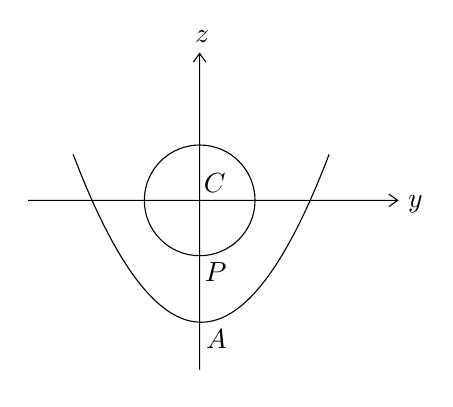
\begin{tikzpicture}[x=0.45pt,y=0.45pt,yscale=-1,xscale=1]
						%uncomment if require: \path (0,523); %set diagram left start at 0, and has height of 523

						%Shape: Axis 2D [id:dp5862780090842503] 
						\draw  (184,368.61) -- (480.67,368.61)(321.67,250.61) -- (321.67,504.61) (473.67,363.61) -- (480.67,368.61) -- (473.67,373.61) (316.67,257.61) -- (321.67,250.61) -- (326.67,257.61)  ;
						%Shape: Circle [id:dp4477394637040828] 
						\draw   (277.22,368.61) .. controls (277.22,344.07) and (297.12,324.17) .. (321.67,324.17) .. controls (346.21,324.17) and (366.11,344.07) .. (366.11,368.61) .. controls (366.11,393.16) and (346.21,413.06) .. (321.67,413.06) .. controls (297.12,413.06) and (277.22,393.16) .. (277.22,368.61) -- cycle ;
						%Shape: Parabola [id:dp9211055614957724] 
						\draw   (220,331.5) .. controls (288.56,511.5) and (357.11,511.5) .. (425.67,331.5) ;

						% Text Node
						\draw (487,362.4) node [anchor=north west][inner sep=0.75pt]    {$y$};
						% Text Node
						\draw (316,230.4) node [anchor=north west][inner sep=0.75pt]    {$z$};
						% Text Node
						\draw (323,345) node [anchor=north west][inner sep=0.75pt]    {$C$};
						% Text Node
						\draw (323.67,416.46) node [anchor=north west][inner sep=0.75pt]    {$P$};
						% Text Node
						\draw (324.83,469.9) node [anchor=north west][inner sep=0.75pt]    {$A$};
				\end{tikzpicture}
				\caption{$z$轴上各点之间关系}
				\label{parabola}
		\end{minipage}
		\begin{minipage}[c]{0.4\textwidth}
				\centering
				\tikzset{every picture/.style={line width=0.75pt}} %set default line width to 0.75pt        

				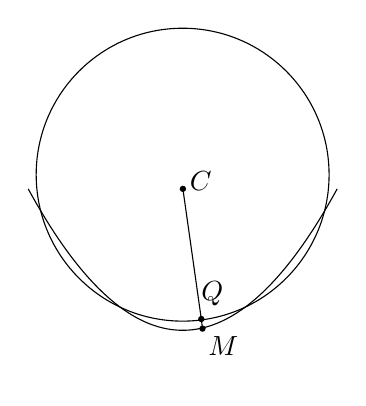
\begin{tikzpicture}[x=0.56pt,y=0.56pt,yscale=-1,xscale=1]
						%uncomment if require: \path (0,352); %set diagram left start at 0, and has height of 352

						%Shape: Circle [id:dp29509496211422026] 
						\draw   (75.33,190.83) .. controls (75.33,138.64) and (117.64,96.33) .. (169.83,96.33) .. controls (222.02,96.33) and (264.33,138.64) .. (264.33,190.83) .. controls (264.33,243.02) and (222.02,285.33) .. (169.83,285.33) .. controls (117.64,285.33) and (75.33,243.02) .. (75.33,190.83) -- cycle ;
						%Shape: Parabola [id:dp0617345337706261] 
						\draw   (70.2,200.01) .. controls (136.64,321.66) and (203.08,321.66) .. (269.53,200.01) ;
						%Straight Lines [id:da9676634590003081] 
						\draw    (170,199.98) -- (181.88,283.97) ;
						\draw [shift={(170,199.98)}, rotate = 81.95] [color={rgb, 255:red, 0; green, 0; blue, 0 }  ][fill={rgb, 255:red, 0; green, 0; blue, 0 }  ][line width=0.75]      (0, 0) circle [x radius= 1.34, y radius= 1.34]   ;
						%Straight Lines [id:da4042056024919958] 
						\draw    (181.88,283.97) -- (182.67,290.15) ;
						\draw [shift={(182.67,290.15)}, rotate = 82.73] [color={rgb, 255:red, 0; green, 0; blue, 0 }  ][fill={rgb, 255:red, 0; green, 0; blue, 0 }  ][line width=0.75]      (0, 0) circle [x radius= 1.34, y radius= 1.34]   ;
						\draw [shift={(181.88,283.97)}, rotate = 82.73] [color={rgb, 255:red, 0; green, 0; blue, 0 }  ][fill={rgb, 255:red, 0; green, 0; blue, 0 }  ][line width=0.75]      (0, 0) circle [x radius= 1.34, y radius= 1.34]   ;

						% Text Node
						\draw (172.73,187.01) node [anchor=north west][inner sep=0.75pt]    {$C$};
						% Text Node
						\draw (180.23,258.42) node [anchor=north west][inner sep=0.75pt]    {$Q$};
						% Text Node
						\draw (184.67,293.55) node [anchor=north west][inner sep=0.75pt]    {$M$};

				\end{tikzpicture}
				\caption{求解伸缩后主索节点坐标}
				\label{CQ}
		\end{minipage}
\end{figure}




\textbf{对于子问题(2)},为求解促动器顶端伸缩后的坐标,可以筛选出可能伸缩到工作态范围内的基准球面上的主索节点,对其中的每一个主索节点$Q$,可确定直线$CQ$,并求出$CQ$与被遍历的抛物面的交点坐标$M$(如\cref{CQ}),即为促动器伸缩后的新主索节点坐标。\par



\textbf{对于子问题(3)},由于主索节点的变化方向是径向的,因此可以认为新旧主索节点坐标之间的距离即为促动器的伸缩量。按照促动器的变化范围要求,可通过判断伸缩量是否在$[-0.6,0.6]$之间来筛选出满足条件的抛物面。通过对不同指标实际意义的比较,本文最终以促动器伸缩量绝对值总和最小为确定最终理想抛物面的指标。

\subsection{问题2的分析:}问题2要求在$\alpha = 36.795^{\circ},\beta= 78.169^{\circ}$的条件下确定理想抛物面。注意到旋转抛物面沿轴的对称性,本文考虑在原始坐标系与以$SC$为$z$轴的坐标系之间建立一个旋转变换关系(如\cref{round:system}),使得问题2经旋转变换后可转化为问题1的情景,从而求得在新坐标系下的理想抛物面方程和其它待求量。再通过逆向旋转变换,最终得到再原始坐标系下的理想抛物面方程和其它待求量。

\begin{figure}[H]
		\centering




		\tikzset{every picture/.style={line width=0.75pt}} %set default line width to 0.75pt        

		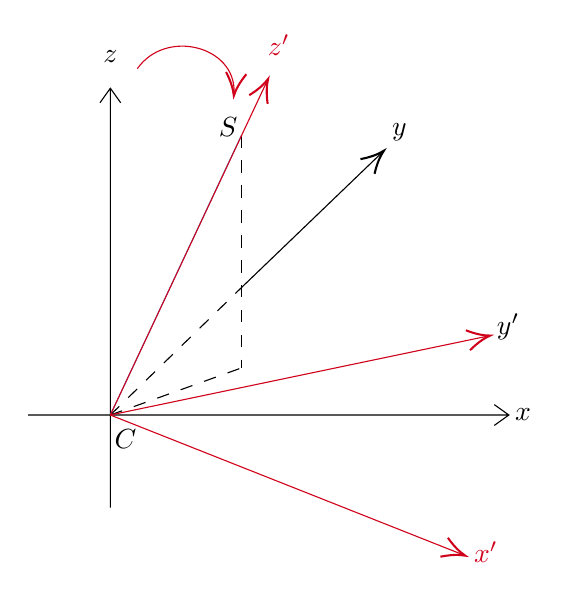
\begin{tikzpicture}[x=0.75pt,y=0.75pt,yscale=-1,xscale=1]
				%uncomment if require: \path (0,373); %set diagram left start at 0, and has height of 373

				%Shape: Axis 2D [id:dp09788258365708624] 
				\draw  (138.44,245.33) -- (370,245.33)(178,87.89) -- (178,290) (363,240.33) -- (370,245.33) -- (363,250.33) (173,94.89) -- (178,87.89) -- (183,94.89)  ;
				%Straight Lines [id:da3567635469042596] 
				\draw [color={rgb, 255:red, 74; green, 144; blue, 226 }  ,draw opacity=1 ]   (178,245.33) -- (241.11,110.67) ;
				%Straight Lines [id:da578064420097069] 
				\draw  [dash pattern={on 4.5pt off 4.5pt}]  (241.11,110.67) -- (241.11,222.67) ;
				%Straight Lines [id:da8679128990173901] 
				\draw  [dash pattern={on 4.5pt off 4.5pt}]  (178,245.33) -- (241.11,222.67) ;
				%Straight Lines [id:da4078152355309548] 
				\draw  [dash pattern={on 4.5pt off 4.5pt}]  (178,245.33) -- (241.11,184) ;
				%Straight Lines [id:da7366378357929284] 
				\draw    (241.11,184) -- (308.34,119.39) ;
				\draw [shift={(309.78,118)}, rotate = 136.13] [color={rgb, 255:red, 0; green, 0; blue, 0 }  ][line width=0.75]    (10.93,-4.9) .. controls (6.95,-2.3) and (3.31,-0.67) .. (0,0) .. controls (3.31,0.67) and (6.95,2.3) .. (10.93,4.9)   ;
				%Straight Lines [id:da4470005379087125] 
				\draw [color={rgb, 255:red, 208; green, 2; blue, 27 }  ,draw opacity=1 ]   (178,245.33) -- (253.15,85.24) ;
				\draw [shift={(254,83.43)}, rotate = 115.15] [color={rgb, 255:red, 208; green, 2; blue, 27 }  ,draw opacity=1 ][line width=0.75]    (10.93,-4.9) .. controls (6.95,-2.3) and (3.31,-0.67) .. (0,0) .. controls (3.31,0.67) and (6.95,2.3) .. (10.93,4.9)   ;
				%Straight Lines [id:da7987238045742824] 
				\draw [color={rgb, 255:red, 208; green, 2; blue, 27 }  ,draw opacity=1 ]   (178,245.33) -- (359.04,207.48) ;
				\draw [shift={(361,207.07)}, rotate = 168.19] [color={rgb, 255:red, 208; green, 2; blue, 27 }  ,draw opacity=1 ][line width=0.75]    (10.93,-4.9) .. controls (6.95,-2.3) and (3.31,-0.67) .. (0,0) .. controls (3.31,0.67) and (6.95,2.3) .. (10.93,4.9)   ;
				%Straight Lines [id:da33533616884876816] 
				\draw [color={rgb, 255:red, 208; green, 2; blue, 27 }  ,draw opacity=1 ]   (178,245.33) -- (347.14,312.35) ;
				\draw [shift={(349,313.08)}, rotate = 201.61] [color={rgb, 255:red, 208; green, 2; blue, 27 }  ,draw opacity=1 ][line width=0.75]    (10.93,-4.9) .. controls (6.95,-2.3) and (3.31,-0.67) .. (0,0) .. controls (3.31,0.67) and (6.95,2.3) .. (10.93,4.9)   ;
				%Curve Lines [id:da5214771876679787] 
				\draw [color={rgb, 255:red, 208; green, 2; blue, 27 }  ,draw opacity=1 ]   (191,78.48) .. controls (204.65,58.98) and (238.26,67.52) .. (237.62,89.74) ;
				\draw [shift={(237.5,91.48)}, rotate = 276.07] [color={rgb, 255:red, 208; green, 2; blue, 27 }  ,draw opacity=1 ][line width=0.75]    (10.93,-4.9) .. controls (6.95,-2.3) and (3.31,-0.67) .. (0,0) .. controls (3.31,0.67) and (6.95,2.3) .. (10.93,4.9)   ;

				% Text Node
				\draw (178.8,251.13) node [anchor=north west][inner sep=0.75pt]    {$C$};
				% Text Node
				\draw (371.73,241.05) node [anchor=north west][inner sep=0.75pt]    {$x$};
				% Text Node
				\draw (312.53,103.85) node [anchor=north west][inner sep=0.75pt]    {$y$};
				% Text Node
				\draw (173.33,68.65) node [anchor=north west][inner sep=0.75pt]    {$z$};
				% Text Node
				\draw (229.03,100.75) node [anchor=north west][inner sep=0.75pt]    {$S$};
				% Text Node
				\draw (252.6,61.05) node [anchor=north west][inner sep=0.75pt]  [color={rgb, 255:red, 208; green, 2; blue, 27 }  ,opacity=1 ]  {$z^{\prime }$};
				% Text Node
				\draw (352,305.07) node [anchor=north west][inner sep=0.75pt]    {$\textcolor[rgb]{0.82,0.01,0.11}{x}\textcolor[rgb]{0.82,0.01,0.11}{^{\prime }}$};
				% Text Node
				\draw (363,195.07) node [anchor=north west][inner sep=0.75pt]    {$y^{\prime }$};


		\end{tikzpicture}
		\caption{新旧坐标系的旋转变换关系}
		\label{round:system}
\end{figure}

\subsection{问题3的分析:}问题3要求在问题2情况下馈源舱的接收比,并与基准态球面的接收比做比较。本文拟采用蒙特卡罗方法,在问题2新建的坐标系下研究,取一条工作态范围内竖直向下的入射光线,通过它和与之对应的反射面三角形所在平面的几何关系获得反射光线,再与馈源舱所在的平行于$xOy$的平面获得交点,观察其是否处在馈源舱的有效区域内。该流程经过大量试验后即可获得接收比。



\section{符号说明}
\begin{center}
		\begin{tabular}{ccc}
				\hline
				\makebox[0.3\textwidth][c]{符号}	& 
				\makebox[0.4\textwidth][c]{说明}	&
				\makebox[0.3\textwidth][c]{单位} \\ \hline
				$S$	     & 被观测体        		    &    \\ 
				$C$	     & 基准球面的球心   		 &    \\ 
				$P$	     & 馈源舱接收平面中心点      &    \\
				$R$	     & 基准球面半径        	  & $m$ \\
				$r$		 & 工作态范围半径			 & $m$  \\
				$F$	     & 基准球面与交面半径之差     & $m$   \\ 
				$D$	     & FAST反射面口径          & $m$   \\
				$p$      & 馈源舱接收圆盘半径		& $m$  \\
				$d$      & 单个促动器伸缩量			 & $m$	\\
				$\Sigma$ & 工作态内所有促动器伸缩量绝对值总和   & $m$	\\
				$\alpha$ & 天体$S$的方位角  		  & $^\circ$   \\
				$\beta$	 & 天体$S$的仰角            & $^\circ$  \\ \hline
				\\
				\\
				\\
		\end{tabular}
\end{center}


\section{模型假设}
\begin{itemize}
		\item[1.]对问题1和问题2,仅考虑把工作态反射面理想化为一个光滑理想抛物面;
		\item[2.]假设促动器顶端伸缩后相邻主索节点间距离的微小变化幅度小于等于$0.07\%$;
		\item[3.]不考虑反射过程中电磁波的能量损失对信号强度的影响;
		\item[4.]不考虑电磁波的二次反射;
		\item[5.]假设电磁波信号在介质中沿直线传播。
\end{itemize}

\newpage
\section{模型建立与求解}
\subsection{问题1的模型建立与求解}
\subsubsection{旋转抛物面簇的确定}
由题目中的方位角和仰角大小$\alpha = 0^{\circ}$、$\beta = 90^{\circ}$可知,旋转抛物面对应的旋转轴即为$z$轴,因此设其方程为$z = a(x^2 + y^2)+b$。根据旋转抛物面的对称性质,本文取$yOz$平面与抛物面截得的抛物线$z = ay^2+b$来讨论,实现问题的降维。\par

\begin{figure}[H]
		\centering
		\tikzset{every picture/.style={line width=0.75pt}} %set default line width to 0.75pt        
		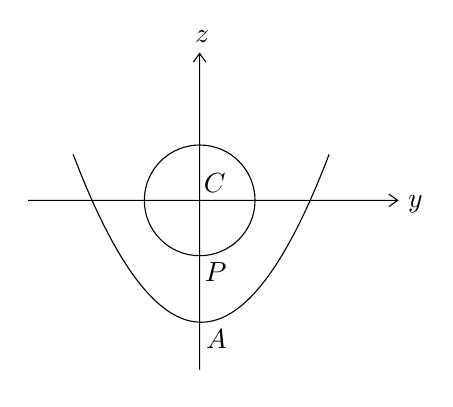
\begin{tikzpicture}[x=0.45pt,y=0.45pt,yscale=-1,xscale=1]
				%uncomment if require: \path (0,523); %set diagram left start at 0, and has height of 523

				%Shape: Axis 2D [id:dp5862780090842503] 
				\draw  (184,368.61) -- (480.67,368.61)(321.67,250.61) -- (321.67,504.61) (473.67,363.61) -- (480.67,368.61) -- (473.67,373.61) (316.67,257.61) -- (321.67,250.61) -- (326.67,257.61)  ;
				%Shape: Circle [id:dp4477394637040828] 
				\draw   (277.22,368.61) .. controls (277.22,344.07) and (297.12,324.17) .. (321.67,324.17) .. controls (346.21,324.17) and (366.11,344.07) .. (366.11,368.61) .. controls (366.11,393.16) and (346.21,413.06) .. (321.67,413.06) .. controls (297.12,413.06) and (277.22,393.16) .. (277.22,368.61) -- cycle ;
				%Shape: Parabola [id:dp9211055614957724] 
				\draw   (220,331.5) .. controls (288.56,511.5) and (357.11,511.5) .. (425.67,331.5) ;

				% Text Node
				\draw (487,362.4) node [anchor=north west][inner sep=0.75pt]    {$y$};
				% Text Node
				\draw (316,230.4) node [anchor=north west][inner sep=0.75pt]    {$z$};
				% Text Node
				\draw (323,345) node [anchor=north west][inner sep=0.75pt]    {$C$};
				% Text Node
				\draw (323.67,416.46) node [anchor=north west][inner sep=0.75pt]    {$P$};
				% Text Node
				\draw (324.83,469.9) node [anchor=north west][inner sep=0.75pt]    {$A$};
		\end{tikzpicture}
		\caption{$yOz$平面内的二维直角坐标系}
		\label{yOz}
\end{figure}
如\cref{yOz}所示,本文基于题目中所给出的坐标系,建立$yOz$面上,以$C$为原点的二维直角坐标系,水平向右为$y$轴正向,竖直向上为$z$轴正向。抛物线开口向上并以$z$轴为对称轴,$P$在焦面球与$yOz$面相交的圆周上,是抛物线的焦点,$A$为抛物线的顶点,位于$z$轴的负半轴上。
易知$A$点坐标为$(0,b)$,$b<0$,并且有数量关系:$|CP|$加上基准球面与交面半径之差$F$即为基准球面半径$R$,即
\begin{equation}
		|CP| = (1 - 0.466)R
		\label{cp}
\end{equation}\par 
又根据抛物线的方程和其性质,抛物线焦距$f$满足:
\begin{equation}
		f = \frac{1}{4a}
		\label{f}
\end{equation}\par 
根据$C$、$P$、$A$间的位置关系有:$|b| = |CP| + f$,结合\cref{cp}\cref{f}整理得到抛物线参数$a$、$b$之间的关系:
\begin{equation}
		-b = 0.534R + \frac{1}{4a}
		\label{ab}
\end{equation}\par 
从基准球面调整为工作态抛物面后,由于顶点$A$处的促动器的变化限制,$b$的取值可以确定为$[-R-0.6,-R+0.6]$
,由\cref{ab}即把原抛物线方程转化成了只含单个参数的方程:
\begin{equation}
		z = -\frac{1}{4(b+0.534R)}y^2 + b,\quad  b \in [-301.0 ,-299.8]
		\label{zyb}
\end{equation}\par 
通过$b$值的变化,即可获得对应的旋转抛物面簇,所求的理想抛物面即在该抛物面簇中。因此,\textbf{本文将$b$作为决策变量,对该抛物面簇进行优化。}
\subsubsection{单目标优化模型的建立}
本文根据理想抛物面的要求,以工作态内所有促动器伸缩量在$[-0.6,0.6]$之间为约束条件,工作态内所有促动器伸缩量绝对值总和$\Sigma$最小为优化目标,建立单目标单变量优化模型。设变化前位于基准球面上的主索节点坐标为$(x_0,y_0,z_0)$,沿径向变化后的工作态抛物面上的新的坐标为$(x_1,y_1,z_1)$。\par 
注意到$\sqrt{x_0^2 + y_0^2 + z_0^2} = R$,\textbf{得出目标函数如下:}
\begin{equation}
		\Sigma = \sum |R - \sqrt{x_1^2 + y_1^2 + z_1^2}|,
		\quad \forall (x_1,y_1,z_1)|x_1^2 + y_1^2 \leq r^2
		\label{sumabs}
\end{equation}\par 
约束条件为:
\begin{equation}
		s.t.  \quad - 0.6 \leq R - \sqrt{x_1^2 + y_1^2 + z_1^2} \leq 0.6, \quad \forall (x_1,y_1,z_1)|x_1^2 + y_1^2 \leq r^2
		\label{st}
\end{equation}\par 
由于工作态内的点太多,以上的约束条件将需要对大量的数据进行处理,降低程序的运行效率,因此拟对该\textbf{约束条件进行改进}。
本文从抛物线的性质出发,获得抛物线上的动点到原点的距离变化关系,总结获得\cref{ltoC}并给出相应的\cref{ptoC}:\\

\begin{lemma}
		对于抛物线方程$z = ay^2 + b$,$a>0$,$b<0$,且$b < -\frac{1}{2a}$。当动点在抛物线上从顶点A沿着一边运动时,其与原点的距离先减小后增大,并在$z = -\frac{1}{2a}$ 处取得最小值。\\
		\label{ltoC}
\end{lemma}

\begin{proof}
		设动点坐标为$(y_0,z_0)$,到原点$C$的距离的平方满足$d_0^2 = y_0^2 + z_0^2$,和抛物线方程联立得:
		$d_0^2 = z_0^2 + \frac{1}{a}z_0 - \frac{b}{a}$,根据二次函数性质得知$d_0$在$z = -\frac{1}{2a}$处取最小值,当动点在抛物线上从顶点A沿着一边运动时,其与原点的距离先减小后增大,证毕。\\
		\label{ptoC}
\end{proof}\par 
根据\cref{AMNC},以下对题中所给信息是否满足\cref{ltoC}的条件展开讨论:\par 
1)首先讨论$b < -\frac{1}{2a}$是否成立。因为$b \in [-301.0 ,-299.8]$,
根据$a$、$b$间的函数关系即公式\cref{ab}可以得到$-\frac{1}{2a} \in (-281.2, -278.7)$;
所以理想抛物面必满足$b < -\frac{1}{2a}$。\par
2)判断工作态边界圈,即$x^2 + y^2 = r^2$与工作态抛物面相交的圆圈所在的面高度$z_{\rm{bound}}$与面$z = -\frac{1}{2a}$的大小关系。根据抛物面方程$z = a(x^2 + y^2)+b$可得出边界圈满足$z_{\rm{bound}} = ar^2 + b$,将公式\cref{ab}代入得到
\begin{equation}
		z_{\rm{bound}} = b - \frac{r^2}{4(b + 0.534R)}
		\label{bound}
\end{equation}\par 
再由$b$的取值范围得到$z_{\rm{bound}} \in (-261.1, -259.4)$,满足$ -\frac{1}{2a} < z_{\rm{bound}}$。


\begin{figure}[H]
		\centering

		\tikzset{every picture/.style={line width=0.75pt}} %set default line width to 0.75pt        

		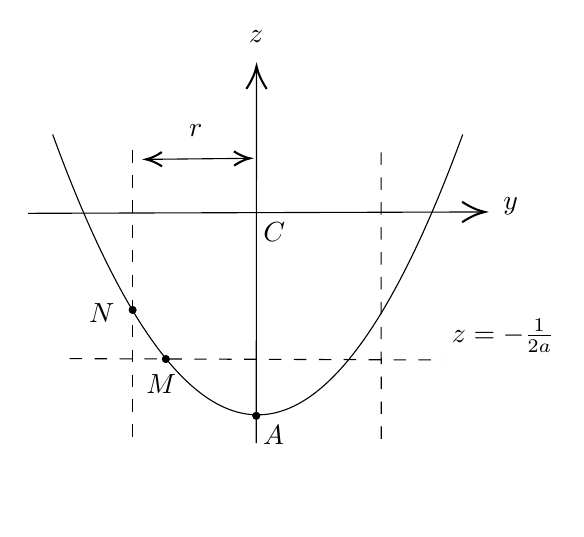
\begin{tikzpicture}[x=0.75pt,y=0.75pt,yscale=-1,xscale=1]
				%uncomment if require: \path (0,300); %set diagram left start at 0, and has height of 300

				%Straight Lines [id:da5850681469003021] 
				\draw    (200.22,71.69) -- (200.06,251.34) ;
				\draw [shift={(200.22,69.69)}, rotate = 90.05] [color={rgb, 255:red, 0; green, 0; blue, 0 }  ][line width=0.75]    (10.93,-4.9) .. controls (6.95,-2.3) and (3.31,-0.67) .. (0,0) .. controls (3.31,0.67) and (6.95,2.3) .. (10.93,4.9)   ;
				%Shape: Parabola [id:dp15684520318138095] 
				\draw   (102,102.58) .. controls (167.85,282.7) and (233.7,282.7) .. (299.56,102.58) ;
				%Straight Lines [id:da38830353347239277] 
				\draw  [dash pattern={on 4.5pt off 4.5pt}]  (110.22,210.58) -- (290.22,211.24) ;
				%Straight Lines [id:da6297030806956725] 
				\draw    (90.22,140.58) -- (308.22,139.92) ;
				\draw [shift={(310.22,139.91)}, rotate = 179.83] [color={rgb, 255:red, 0; green, 0; blue, 0 }  ][line width=0.75]    (10.93,-4.9) .. controls (6.95,-2.3) and (3.31,-0.67) .. (0,0) .. controls (3.31,0.67) and (6.95,2.3) .. (10.93,4.9)   ;
				%Straight Lines [id:da3217724091325418] 
				\draw  [dash pattern={on 4.5pt off 4.5pt}]  (140.3,110.27) -- (140.3,250.27) ;
				%Straight Lines [id:da6536863113188589] 
				\draw  [dash pattern={on 4.5pt off 4.5pt}]  (260.22,111.24) -- (260.3,250.94) ;
				%Straight Lines [id:da037473075189077276] 
				\draw    (149,114.56) -- (195,114.1) ;
				\draw [shift={(197,114.08)}, rotate = 179.43] [color={rgb, 255:red, 0; green, 0; blue, 0 }  ][line width=0.75]    (7.65,-3.43) .. controls (4.86,-1.61) and (2.31,-0.47) .. (0,0) .. controls (2.31,0.47) and (4.86,1.61) .. (7.65,3.43)   ;
				\draw [shift={(147,114.58)}, rotate = 359.43] [color={rgb, 255:red, 0; green, 0; blue, 0 }  ][line width=0.75]    (7.65,-3.43) .. controls (4.86,-1.61) and (2.31,-0.47) .. (0,0) .. controls (2.31,0.47) and (4.86,1.61) .. (7.65,3.43)   ;
				%Straight Lines [id:da5497534039397212] 
				\draw    (140.52,187.13) ;
				\draw [shift={(140.52,187.13)}, rotate = 0] [color={rgb, 255:red, 0; green, 0; blue, 0 }  ][fill={rgb, 255:red, 0; green, 0; blue, 0 }  ][line width=0.75]      (0, 0) circle [x radius= 1.34, y radius= 1.34]   ;
				\draw [shift={(140.52,187.13)}, rotate = 0] [color={rgb, 255:red, 0; green, 0; blue, 0 }  ][fill={rgb, 255:red, 0; green, 0; blue, 0 }  ][line width=0.75]      (0, 0) circle [x radius= 1.34, y radius= 1.34]   ;
				%Straight Lines [id:da2563058132246605] 
				\draw    (156.52,210.79) ;
				\draw [shift={(156.52,210.79)}, rotate = 0] [color={rgb, 255:red, 0; green, 0; blue, 0 }  ][fill={rgb, 255:red, 0; green, 0; blue, 0 }  ][line width=0.75]      (0, 0) circle [x radius= 1.34, y radius= 1.34]   ;
				\draw [shift={(156.52,210.79)}, rotate = 0] [color={rgb, 255:red, 0; green, 0; blue, 0 }  ][fill={rgb, 255:red, 0; green, 0; blue, 0 }  ][line width=0.75]      (0, 0) circle [x radius= 1.34, y radius= 1.34]   ;
				%Straight Lines [id:da09966174913703152] 
				\draw    (200.08,238.15) ;
				\draw [shift={(200.08,238.15)}, rotate = 0] [color={rgb, 255:red, 0; green, 0; blue, 0 }  ][fill={rgb, 255:red, 0; green, 0; blue, 0 }  ][line width=0.75]      (0, 0) circle [x radius= 1.34, y radius= 1.34]   ;
				\draw [shift={(200.08,238.15)}, rotate = 0] [color={rgb, 255:red, 0; green, 0; blue, 0 }  ][fill={rgb, 255:red, 0; green, 0; blue, 0 }  ][line width=0.75]      (0, 0) circle [x radius= 1.34, y radius= 1.34]   ;

				% Text Node
				\draw (202.08,241.55) node [anchor=north west][inner sep=0.75pt]    {$A$};
				% Text Node
				\draw (166.5,96.57) node [anchor=north west][inner sep=0.75pt]    {$r$};
				% Text Node
				\draw (293.08,190.35) node [anchor=north west][inner sep=0.75pt]    {$z=-\frac{1}{2a}$};
				% Text Node
				\draw (145.85,216.86) node [anchor=north west][inner sep=0.75pt]    {$M$};
				% Text Node
				\draw (118.29,183.02) node [anchor=north west][inner sep=0.75pt]    {$N$};
				% Text Node
				\draw (195.33,51.4) node [anchor=north west][inner sep=0.75pt]    {$z$};
				% Text Node
				\draw (317.89,131.64) node [anchor=north west][inner sep=0.75pt]    {$y$};
				% Text Node
				\draw (202.22,143.64) node [anchor=north west][inner sep=0.75pt]    {$C$};


		\end{tikzpicture}
		\caption{抛物线上$A$、$M$、$N$与原点$C$的位置关系}
		\label{AMNC}
\end{figure}
如\cref{AMNC}所示,$A$点为抛物线的顶点,$M$是抛物线上$z$坐标为$ -\frac{1}{2a} $的点,$N$则是距离$z$轴为$r$的点,即工作态边界点,所以根据\cref{ltoC}有:动点在抛物线上从$A$出发,向着$y$坐标减小的方向运动,在$AM$段与原点$C$的距离逐渐减小,在$M$处取得最小值,在$MN$段逐渐增大。结合抛物面方程$z = a(x^2 + y^2)+b$,在曲线$AN$段上有:\\
对于$M$满足$z_M = -\frac{1}{2a}$时有$|MC|$最小:
\begin{equation}
		|MC| = \sqrt{x_M^2 + y_M^2 + z_M^2} = \sqrt{z_M^2 + \frac{1}{a}z_M - \frac{b}{a}}
		= \sqrt{-\frac{1}{4a^2} - \frac{b}{a}}
		\label{dm}
\end{equation}\par 
对于$N$满足$x_N^2 + y_N^2 = r^2$有$|NC|$为边界极值:
\begin{equation}
		|NC| = \sqrt{x_N^2 + y_N^2 + z_N^2} = \sqrt{r^2 + (ar^2 + b)^2}
		\label{dn}
\end{equation}\par 
由\cref{dm}\cref{dn},本文把先前的约束条件\cref{st}改进为:
\begin{equation}
		s.t.  \quad  \begin{cases}
				d_{\rm{min}} = \sqrt{-\frac{1}{4a^2} - \frac{b}{a}} - R \geq -0.6\\

				d_{\rm{max}} = \sqrt{r^2 + (ar^2 + b)^2} - R \leq 0.6
		\end{cases}
		\label{newst}
\end{equation}\par 
大幅度降低了对约束条件的判断复杂度。
\subsubsection{单目标优化模型的求解}
本文建立的\textbf{基于变步长遍历计算}的单目标优化模型求解算法步骤如下:\par 
1)\textbf{预处理}:设置半径$R = 300.4m$,工作态边界半径$r = 300m \times 0.5 = 150m$。加载数据\texttt{附件1.csv},获取所有可能伸缩到工作态$300m$口径内的点。由于在基准球面中$x^2 + y^2$略大于$r^2$的点也可能在工作态时收缩到$300m$口径内,因此本文以满足$x^2 + y^2 \leq (r+0.6)^2$为筛选条件对数据进行筛选。\par 
\newpage
2)\textbf{遍历求得目标函数}:以$b$为决策变量,设置步长为$0.01$,对抛物面簇进行遍历寻优:\\
对于$b$的每一次取值,都有一个确定的抛物面$S_0$与之对应。先利用约束条件\cref{newst}筛选掉不符合促动器伸缩量在$[-0.6,0.6]$的抛物面。
再求第一步预处理后的点移动到工作态抛物面后的新的坐标,进而求促动器的伸缩量,并且对于每个$b$都要初始化工作态内所有促动器伸缩量绝对值总和$\Sigma$为$0$。以下开始对这些点进行遍历:\\
\begin{figure}[H]
		\centering
		\tikzset{every picture/.style={line width=0.75pt}} %set default line width to 0.75pt        

		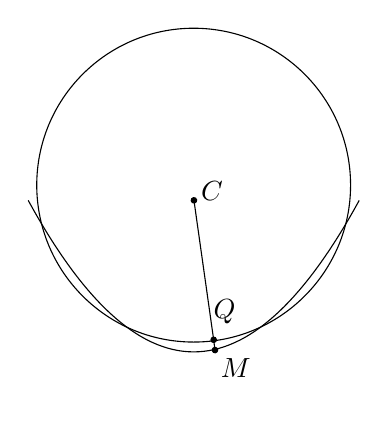
\begin{tikzpicture}[x=0.60pt,y=0.60pt,yscale=-1,xscale=1]
				%uncomment if require: \path (0,352); %set diagram left start at 0, and has height of 352

				%Shape: Circle [id:dp29509496211422026] 
				\draw   (75.33,190.83) .. controls (75.33,138.64) and (117.64,96.33) .. (169.83,96.33) .. controls (222.02,96.33) and (264.33,138.64) .. (264.33,190.83) .. controls (264.33,243.02) and (222.02,285.33) .. (169.83,285.33) .. controls (117.64,285.33) and (75.33,243.02) .. (75.33,190.83) -- cycle ;
				%Shape: Parabola [id:dp0617345337706261] 
				\draw   (70.2,200.01) .. controls (136.64,321.66) and (203.08,321.66) .. (269.53,200.01) ;
				%Straight Lines [id:da9676634590003081] 
				\draw    (170,199.98) -- (181.88,283.97) ;
				\draw [shift={(170,199.98)}, rotate = 81.95] [color={rgb, 255:red, 0; green, 0; blue, 0 }  ][fill={rgb, 255:red, 0; green, 0; blue, 0 }  ][line width=0.75]      (0, 0) circle [x radius= 1.34, y radius= 1.34]   ;
				%Straight Lines [id:da4042056024919958] 
				\draw    (181.88,283.97) -- (182.67,290.15) ;
				\draw [shift={(182.67,290.15)}, rotate = 82.73] [color={rgb, 255:red, 0; green, 0; blue, 0 }  ][fill={rgb, 255:red, 0; green, 0; blue, 0 }  ][line width=0.75]      (0, 0) circle [x radius= 1.34, y radius= 1.34]   ;
				\draw [shift={(181.88,283.97)}, rotate = 82.73] [color={rgb, 255:red, 0; green, 0; blue, 0 }  ][fill={rgb, 255:red, 0; green, 0; blue, 0 }  ][line width=0.75]      (0, 0) circle [x radius= 1.34, y radius= 1.34]   ;

				% Text Node
				\draw (172.73,187.01) node [anchor=north west][inner sep=0.75pt]    {$C$};
				% Text Node
				\draw (180.23,258.42) node [anchor=north west][inner sep=0.75pt]    {$Q$};
				% Text Node
				\draw (184.67,293.55) node [anchor=north west][inner sep=0.75pt]    {$M$};


		\end{tikzpicture}
		\caption{求解促动器伸缩后的主索节点坐标}
		\label{CQM}
\end{figure}

如\cref{CQM}所示,设该基准球面上的主索节点坐标为$Q(x_Q,y_Q,z_Q)$,沿径向伸缩后落在抛物面$S_0$的$M$上。联立
\begin{equation}
		\begin{cases}
				l_{CQ}: \frac{x}{x_Q} = \frac{y}{y_Q} = \frac{z}{z_Q} \\
				S_0:  z = a(x^2 + y^2) + b
		\end{cases}
\end{equation}\par 
解得$M$的坐标$(x_M,y_M,z_M)$,根据相似三角形的原理,计算其促动器伸缩量$d_M$:
\begin{equation}
		d_M = (\frac{z_M}{z_Q} - 1)R
\end{equation}\par 
若$M$在工作态范围内,目标函数$\Sigma$加上$d_M$的绝对值:
\begin{equation}
		\Sigma = \sum |d_M|, \quad  \forall M(x_M,y_M,z_M)|x_M^2 + y_M^2 \leq r^2
\end{equation}\par 
遍历决策变量范围内所有的值之后,即可获得$(b,\Sigma)$之间的键值对关系。\par 
3)\textbf{变步长与结果分析}:在这些键值对关系中,通过简单比较即可获得最小的目标函数$\Sigma_{\rm{min}}$,记录对应步长的最优解$b_{\rm{best}}$。在下一轮中缩小决策变量区间,分别更换遍历步长为$0.001$、$0.0001$,最终本文确定的理想抛物面为:
\[
		\bm{z = 0.0017795(x^2+y^2)-300.9017 }
\]\\

\subsection{问题2的模型建立与求解}

\subsubsection{模型准备}
\begin{figure}[H]
		\centering


		\tikzset{every picture/.style={line width=0.75pt}} %set default line width to 0.75pt        

		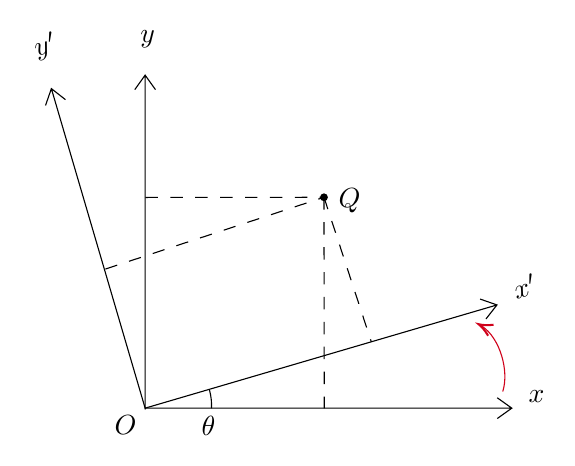
\begin{tikzpicture}[x=0.75pt,y=0.75pt,yscale=-1,xscale=1]
				%uncomment if require: \path (0,300); %set diagram left start at 0, and has height of 300

				%Shape: Axis 2D [id:dp6621525035441915] 
				\draw  (124,221.45) -- (300.67,221.45)(124,61) -- (124,222) (293.67,216.45) -- (300.67,221.45) -- (293.67,226.45) (119,68) -- (124,61) -- (129,68)  ;
				%Shape: Axis 2D [id:dp11301190181738274] 
				\draw  (124,221.45) -- (293.52,171.72)(78.83,67.49) -- (124.16,221.98) (285.4,168.89) -- (293.52,171.72) -- (288.21,178.48) (76.01,75.61) -- (78.83,67.49) -- (85.6,72.8)  ;
				%Straight Lines [id:da04935967028502364] 
				\draw  [dash pattern={on 4.5pt off 4.5pt}]  (210.17,119.85) -- (210.3,221.6) ;
				\draw [shift={(210.17,119.85)}, rotate = 89.93] [color={rgb, 255:red, 0; green, 0; blue, 0 }  ][fill={rgb, 255:red, 0; green, 0; blue, 0 }  ][line width=0.75]      (0, 0) circle [x radius= 1.34, y radius= 1.34]   ;
				%Straight Lines [id:da16711452732631216] 
				\draw  [dash pattern={on 4.5pt off 4.5pt}]  (124.13,119.93) -- (210.17,119.85) ;
				%Straight Lines [id:da2752040089535581] 
				\draw  [dash pattern={on 4.5pt off 4.5pt}]  (210.17,119.85) -- (232.96,189.47) ;
				%Straight Lines [id:da2676334759739516] 
				\draw  [dash pattern={on 4.5pt off 4.5pt}]  (104.84,154.43) -- (210.17,119.85) ;
				%Curve Lines [id:da6992150429948718] 
				\draw [color={rgb, 255:red, 208; green, 2; blue, 27 }  ,draw opacity=1 ]   (296.3,213.42) .. controls (299.43,203.6) and (295.1,187.9) .. (286.39,182) ;
				\draw [shift={(284.67,181)}, rotate = 26.28] [color={rgb, 255:red, 208; green, 2; blue, 27 }  ,draw opacity=1 ][line width=0.75]    (6.56,-2.94) .. controls (4.17,-1.38) and (1.99,-0.4) .. (0,0) .. controls (1.99,0.4) and (4.17,1.38) .. (6.56,2.94)   ;
				%Shape: Arc [id:dp8714849629065915] 
				\draw  [draw opacity=0] (155.03,212.78) .. controls (155.8,215.68) and (156.11,218.64) .. (156,221.55) -- (126.23,220.18) -- cycle ; \draw   (155.03,212.78) .. controls (155.8,215.68) and (156.11,218.64) .. (156,221.55) ;  

				% Text Node
				\draw (108,223.9) node [anchor=north west][inner sep=0.75pt]    {$O$};
				% Text Node
				\draw (307.5,211.9) node [anchor=north west][inner sep=0.75pt]    {$x$};
				% Text Node
				\draw (120.5,38.4) node [anchor=north west][inner sep=0.75pt]    {$y$};
				% Text Node
				\draw (298.53,158.82) node [anchor=north west][inner sep=0.75pt]  [rotate=-343.76]  {$x^{\prime }$};
				% Text Node
				\draw (67.68,41.58) node [anchor=north west][inner sep=0.75pt]  [rotate=-345.25]  {$y^{\prime }$};
				% Text Node
				\draw (150,224.2) node [anchor=north west][inner sep=0.75pt]    {$\theta $};
				% Text Node
				\draw (216,114.51) node [anchor=north west][inner sep=0.75pt]    {$Q$};


		\end{tikzpicture}
		\caption{二维坐标系旋转推导}
		\label{rotation_two}
\end{figure}

1)旋转矩阵\par 



如\cref{rotation_two}所示,考虑二维坐标系旋转,设点$Q$在坐标系$xOy$中的坐标为$(x,y)$,在相对$xOy$逆时针旋转$\theta$角后的新坐标系$x^{\prime}Oy^{\prime}$中的坐标为$(x^{\prime},y^{\prime})$。根据图中的几何关系,满足
\[
		\begin{cases}

				x^{\prime} = x~{\rm cos}\theta + y~{\rm sin} \theta\\ 

				y^{\prime} = y~{\rm cos}\theta - x~{\rm sin} \theta

		\end{cases}
\]
\par
转化为矩阵形式表示即为
\[
		\left(
				\begin{array}{c}
						x^{\prime} \\
						y^{\prime}
				\end{array}
		\right)
		=
		\left(
				\begin{array} {cc}
						{\rm cos}\theta & {\rm sin} \theta \\
						-{\rm sin}\theta& {\rm cos} \theta  
				\end{array}
		\right)
		\left(
				\begin{array}c
						x \\
						y
				\end{array}
		\right)
\]\par
故坐标系$x^{\prime}Oy^{\prime}$相对于坐标系$xOy$的旋转变换矩阵为$\left(
		\begin{array} {cc}
				{\rm cos}\theta & {\rm sin} \theta \\
				-{\rm sin}\theta& {\rm cos} \theta  
		\end{array}
\right)$,它可以将坐标系$xOy$下的向量映射为坐标系$x^{\prime}Oy^{\prime}$下的对应向量。\par 
类似地,考虑三维坐标系下绕单坐标轴的旋转。不妨假设坐标系$xOy$绕坐标轴$z$逆时针旋转$\theta$角变为坐标系$x^{\prime}Oy^{\prime}$,由于$z$轴固定,故$z$坐标不变,而$xOy$平面绕原点逆时针旋转了$\theta$角,与\cref{rotation_two}所示情景完全相同,故满足
\[
		\begin{cases}
				x^{\prime} = x~{\rm cos}\theta + y~{\rm sin} \theta  \\
				y^{\prime} = y~{\rm cos}\theta - x~{\rm sin} \theta   \\
				z^{\prime} = z
		\end{cases}
\]

\par 
即可导出对应的旋转矩阵为
$
\left(
		\begin{array}{ccc}
				{\rm cos}\theta & {\rm sin} \theta & 0\\
				-{\rm sin}\theta& {\rm cos}\theta & 0\\
				0&0&1
		\end{array}
\right)
$。
\par
由于三维坐标系的任意旋转等价于三维坐标系绕单坐标轴的旋转的组合,因此对应的旋转矩阵即可表示为若干三维坐标系绕单坐标轴旋转的旋转矩阵的乘积。

\begin{figure}[H]
		\centering




		\tikzset{every picture/.style={line width=0.75pt}} %set default line width to 0.75pt        

		\begin{tikzpicture}[x=1.2pt,y=1.2pt,yscale=-1,xscale=1]
				%uncomment if require: \path (0,300); %set diagram left start at 0, and has height of 300

				%Shape: Arc [id:dp2698032405438162] 
				\draw  [draw opacity=0] (225.98,184.92) .. controls (215.58,217.02) and (185.54,240.23) .. (150.1,240.23) .. controls (114.63,240.23) and (84.56,216.98) .. (74.19,184.83) -- (150.1,160.12) -- cycle ; \draw   (225.98,184.92) .. controls (215.58,217.02) and (185.54,240.23) .. (150.1,240.23) .. controls (114.63,240.23) and (84.56,216.98) .. (74.19,184.83) ;  
				%Straight Lines [id:da18558291198747323] 
				\draw    (150.2,240.25) ;
				\draw [shift={(150.2,240.25)}, rotate = 0] [color={rgb, 255:red, 0; green, 0; blue, 0 }  ][fill={rgb, 255:red, 0; green, 0; blue, 0 }  ][line width=0.75]      (0, 0) circle [x radius= 1.34, y radius= 1.34]   ;
				\draw [shift={(150.2,240.25)}, rotate = 0] [color={rgb, 255:red, 0; green, 0; blue, 0 }  ][fill={rgb, 255:red, 0; green, 0; blue, 0 }  ][line width=0.75]      (0, 0) circle [x radius= 1.34, y radius= 1.34]   ;
				%Straight Lines [id:da08401261965979745] 
				\draw    (109.09,228.92) ;
				\draw [shift={(109.09,228.92)}, rotate = 0] [color={rgb, 255:red, 0; green, 0; blue, 0 }  ][fill={rgb, 255:red, 0; green, 0; blue, 0 }  ][line width=0.75]      (0, 0) circle [x radius= 1.34, y radius= 1.34]   ;
				\draw [shift={(109.09,228.92)}, rotate = 0] [color={rgb, 255:red, 0; green, 0; blue, 0 }  ][fill={rgb, 255:red, 0; green, 0; blue, 0 }  ][line width=0.75]      (0, 0) circle [x radius= 1.34, y radius= 1.34]   ;
				%Straight Lines [id:da4573305900547333] 
				\draw    (150.1,160.12) ;
				\draw [shift={(150.1,160.12)}, rotate = 0] [color={rgb, 255:red, 0; green, 0; blue, 0 }  ][fill={rgb, 255:red, 0; green, 0; blue, 0 }  ][line width=0.75]      (0, 0) circle [x radius= 1.34, y radius= 1.34]   ;
				%Straight Lines [id:da48954422305649437] 
				\draw  [dash pattern={on 4.5pt off 4.5pt}]  (150.1,160.12) -- (109.09,228.92) ;
				%Straight Lines [id:da13811281815312548] 
				\draw  [dash pattern={on 4.5pt off 4.5pt}]  (76.41,190.78) -- (117.24,215.28) ;
				\draw [shift={(117.24,215.28)}, rotate = 30.96] [color={rgb, 255:red, 0; green, 0; blue, 0 }  ][fill={rgb, 255:red, 0; green, 0; blue, 0 }  ][line width=0.75]      (0, 0) circle [x radius= 1.34, y radius= 1.34]   ;
				%Straight Lines [id:da0824881408334226] 
				\draw  [dash pattern={on 4.5pt off 4.5pt}]  (76.41,190.78) -- (150.1,160.12) ;
				\draw [shift={(76.41,190.78)}, rotate = 337.41] [color={rgb, 255:red, 0; green, 0; blue, 0 }  ][fill={rgb, 255:red, 0; green, 0; blue, 0 }  ][line width=0.75]      (0, 0) circle [x radius= 1.34, y radius= 1.34]   ;
				%Straight Lines [id:da747990163177805] 
				\draw  [dash pattern={on 4.5pt off 4.5pt}]  (150.1,160.12) -- (150.2,240.25) ;
				%Straight Lines [id:da3680233359553846] 
				\draw  [dash pattern={on 4.5pt off 4.5pt}]  (76.41,190.78) -- (150.24,190.65) ;
				\draw [shift={(150.24,190.65)}, rotate = 359.9] [color={rgb, 255:red, 0; green, 0; blue, 0 }  ][fill={rgb, 255:red, 0; green, 0; blue, 0 }  ][line width=0.75]      (0, 0) circle [x radius= 1.34, y radius= 1.34]   ;
				%Straight Lines [id:da3109248177764081] 
				\draw    (150.1,160.12) -- (192.46,89.09) ;
				\draw [shift={(192.46,89.09)}, rotate = 300.81] [color={rgb, 255:red, 0; green, 0; blue, 0 }  ][fill={rgb, 255:red, 0; green, 0; blue, 0 }  ][line width=0.75]      (0, 0) circle [x radius= 1.34, y radius= 1.34]   ;
				%Straight Lines [id:da8759845306113632] 
				\draw  [dash pattern={on 4.5pt off 4.5pt}]  (150.1,160.12) -- (191.33,160.08) ;
				%Shape: Arc [id:dp7509801050714828] 
				\draw  [draw opacity=0] (159.53,144.59) .. controls (162.98,145.61) and (165.71,147.62) .. (167.15,150.54) .. controls (168.53,153.37) and (168.5,156.63) .. (167.32,159.88) -- (147.33,160.27) -- cycle ; \draw   (159.53,144.59) .. controls (162.98,145.61) and (165.71,147.62) .. (167.15,150.54) .. controls (168.53,153.37) and (168.5,156.63) .. (167.32,159.88) ;  
				%Shape: Arc [id:dp37400685464532546] 
				\draw  [draw opacity=0] (141.24,175.17) .. controls (139.04,173.73) and (136.93,171.48) .. (135.31,168.65) .. controls (134.96,168.03) and (134.64,167.41) .. (134.36,166.78) -- (142.73,164.4) -- cycle ; \draw   (141.24,175.17) .. controls (139.04,173.73) and (136.93,171.48) .. (135.31,168.65) .. controls (134.96,168.03) and (134.64,167.41) .. (134.36,166.78) ;  

				% Text Node
				\draw (136.35,137.31) node [anchor=north west][inner sep=0.75pt]    {$C$};
				% Text Node
				\draw (139.2,244.67) node [anchor=north west][inner sep=0.75pt]    {$A_{0}$};
				% Text Node
				\draw (94,233.27) node [anchor=north west][inner sep=0.75pt]    {$D_{27}$};
				% Text Node
				\draw (60.4,186.47) node [anchor=north west][inner sep=0.75pt]    {$B$};
				% Text Node
				\draw (151.6,183.27) node [anchor=north west][inner sep=0.75pt]    {$E$};
				% Text Node
				\draw (118.4,210.87) node [anchor=north west][inner sep=0.75pt]    {$G$};
				% Text Node
				\draw (197,77.9) node [anchor=north west][inner sep=0.75pt]    {$S$};
				% Text Node
				\draw (170.92,141.51) node [anchor=north west][inner sep=0.75pt]    {$\beta $};
				% Text Node
				\draw (128.22,170.51) node [anchor=north west][inner sep=0.75pt]    {$\gamma $};


		\end{tikzpicture}
		\caption{抛物面边界点几何关系}
		\label{verification}
\end{figure}	
2)边界判断
\par 
如\cref{verification}所示,$300$米口径的旋转抛物面有可能超出主动反射面的边界,为对此作出判断,需要计算旋转抛物面边界点$B$到主动反射面中轴$CA_0$的距离$BE$,并与主动反射面的开口半径进行比较。\par 

由于促动器顶端的伸缩量远小于主动反射面的半径,在计算$BE$时可忽略主索节点的微小移动,把旋转抛物面近似为基准球面计算。\par

根据 \cref{verification} 所示的几何关系,满足
\[
		{\rm sin}\gamma = \frac{BG}{BC} =\frac{150}{300}=\frac{1}{2}
\]
\[
		\beta + \angle A_0CD_{27} = 90^{\circ}
\]

\par
解得
\[
		\begin{cases}
				\gamma = 30^{\circ}\\
				\angle A_0CD_{27} = 11.831^{\circ}
		\end{cases}
\]

故
\[
		\angle BCE = \gamma + \angle A_0CD_{27} = 41.831^{\circ}
\]
\[
		BE = BC~{\rm sin}\angle BCE = 300.4 \times {\rm sin} 41.831^{\circ} = 200.347<\frac{500}{2}=250
\]
\par
因此,$300$米口径的旋转抛物面边界不会超出主动反射面的边界。








\subsubsection{模型建立}

1)找出待求理想抛物面顶点处的主索节点\par
假设理想抛物面顶点处存在主索节点$M$,根据旋转抛物面的对称性,$M$应位于直线$SC$上。由于促动器顶端只能沿径向伸缩,则$M$在移动前也应位于直线$SC$上,即直线$SC$与基准球面的交点。仍在第一问坐标系下研究,由$\alpha = 36.795^{\circ},\beta= 78.169^{\circ}$可知直线$SC$的参数方程为



\begin{equation}
		l_{SC}:
		\begin{cases}
				x={\rm cos}\beta~ {\rm cos} \alpha~ t   \\
				y={\rm cos}\beta~ {\rm sin} \alpha~ t   \\
				z={\rm sin}\beta~t
		\end{cases}
\end{equation}

代入基准球面方程
\[
		x^2+y^2+z^2=R^2
\]
\par
可解得交点坐标为
\[
		(-49.3200, -36.8894,-294.0185)
\]
\par
\texttt{附件1.csv}中$D_{27}$的坐标为$(-49.3194,-36.889,-294.0187)$,与解出的交点坐标相同,故理想抛物面顶点处存在主索节点$M$的猜想成立,且$M$为$D_{27}$。
\par
\begin{figure}[H]
		\centering




		\tikzset{every picture/.style={line width=0.75pt}} %set default line width to 0.75pt        

		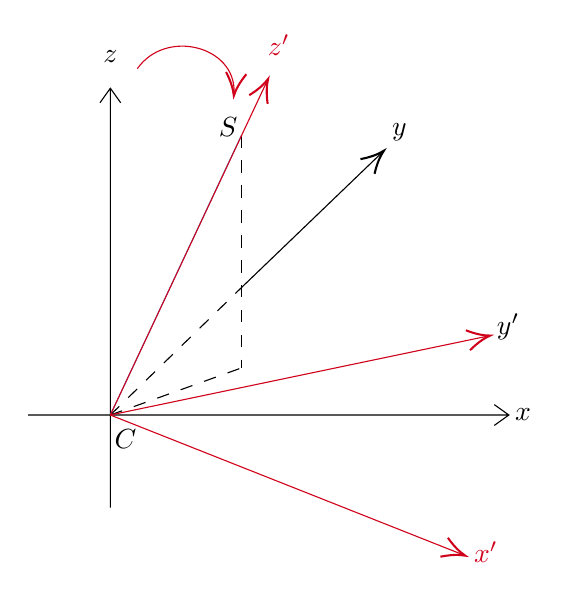
\begin{tikzpicture}[x=0.75pt,y=0.75pt,yscale=-1,xscale=1]
				%uncomment if require: \path (0,373); %set diagram left start at 0, and has height of 373

				%Shape: Axis 2D [id:dp09788258365708624] 
				\draw  (138.44,245.33) -- (370,245.33)(178,87.89) -- (178,290) (363,240.33) -- (370,245.33) -- (363,250.33) (173,94.89) -- (178,87.89) -- (183,94.89)  ;
				%Straight Lines [id:da3567635469042596] 
				\draw [color={rgb, 255:red, 74; green, 144; blue, 226 }  ,draw opacity=1 ]   (178,245.33) -- (241.11,110.67) ;
				%Straight Lines [id:da578064420097069] 
				\draw  [dash pattern={on 4.5pt off 4.5pt}]  (241.11,110.67) -- (241.11,222.67) ;
				%Straight Lines [id:da8679128990173901] 
				\draw  [dash pattern={on 4.5pt off 4.5pt}]  (178,245.33) -- (241.11,222.67) ;
				%Straight Lines [id:da4078152355309548] 
				\draw  [dash pattern={on 4.5pt off 4.5pt}]  (178,245.33) -- (241.11,184) ;
				%Straight Lines [id:da7366378357929284] 
				\draw    (241.11,184) -- (308.34,119.39) ;
				\draw [shift={(309.78,118)}, rotate = 136.13] [color={rgb, 255:red, 0; green, 0; blue, 0 }  ][line width=0.75]    (10.93,-4.9) .. controls (6.95,-2.3) and (3.31,-0.67) .. (0,0) .. controls (3.31,0.67) and (6.95,2.3) .. (10.93,4.9)   ;
				%Straight Lines [id:da4470005379087125] 
				\draw [color={rgb, 255:red, 208; green, 2; blue, 27 }  ,draw opacity=1 ]   (178,245.33) -- (253.15,85.24) ;
				\draw [shift={(254,83.43)}, rotate = 115.15] [color={rgb, 255:red, 208; green, 2; blue, 27 }  ,draw opacity=1 ][line width=0.75]    (10.93,-4.9) .. controls (6.95,-2.3) and (3.31,-0.67) .. (0,0) .. controls (3.31,0.67) and (6.95,2.3) .. (10.93,4.9)   ;
				%Straight Lines [id:da7987238045742824] 
				\draw [color={rgb, 255:red, 208; green, 2; blue, 27 }  ,draw opacity=1 ]   (178,245.33) -- (359.04,207.48) ;
				\draw [shift={(361,207.07)}, rotate = 168.19] [color={rgb, 255:red, 208; green, 2; blue, 27 }  ,draw opacity=1 ][line width=0.75]    (10.93,-4.9) .. controls (6.95,-2.3) and (3.31,-0.67) .. (0,0) .. controls (3.31,0.67) and (6.95,2.3) .. (10.93,4.9)   ;
				%Straight Lines [id:da33533616884876816] 
				\draw [color={rgb, 255:red, 208; green, 2; blue, 27 }  ,draw opacity=1 ]   (178,245.33) -- (347.14,312.35) ;
				\draw [shift={(349,313.08)}, rotate = 201.61] [color={rgb, 255:red, 208; green, 2; blue, 27 }  ,draw opacity=1 ][line width=0.75]    (10.93,-4.9) .. controls (6.95,-2.3) and (3.31,-0.67) .. (0,0) .. controls (3.31,0.67) and (6.95,2.3) .. (10.93,4.9)   ;
				%Curve Lines [id:da5214771876679787] 
				\draw [color={rgb, 255:red, 208; green, 2; blue, 27 }  ,draw opacity=1 ]   (191,78.48) .. controls (204.65,58.98) and (238.26,67.52) .. (237.62,89.74) ;
				\draw [shift={(237.5,91.48)}, rotate = 276.07] [color={rgb, 255:red, 208; green, 2; blue, 27 }  ,draw opacity=1 ][line width=0.75]    (10.93,-4.9) .. controls (6.95,-2.3) and (3.31,-0.67) .. (0,0) .. controls (3.31,0.67) and (6.95,2.3) .. (10.93,4.9)   ;

				% Text Node
				\draw (178.8,251.13) node [anchor=north west][inner sep=0.75pt]    {$C$};
				% Text Node
				\draw (371.73,241.05) node [anchor=north west][inner sep=0.75pt]    {$x$};
				% Text Node
				\draw (312.53,103.85) node [anchor=north west][inner sep=0.75pt]    {$y$};
				% Text Node
				\draw (173.33,68.65) node [anchor=north west][inner sep=0.75pt]    {$z$};
				% Text Node
				\draw (229.03,100.75) node [anchor=north west][inner sep=0.75pt]    {$S$};
				% Text Node
				\draw (252.6,61.05) node [anchor=north west][inner sep=0.75pt]  [color={rgb, 255:red, 208; green, 2; blue, 27 }  ,opacity=1 ]  {$z^{\prime }$};
				% Text Node
				\draw (352,305.07) node [anchor=north west][inner sep=0.75pt]    {$\textcolor[rgb]{0.82,0.01,0.11}{x}\textcolor[rgb]{0.82,0.01,0.11}{^{\prime }}$};
				% Text Node
				\draw (363,195.07) node [anchor=north west][inner sep=0.75pt]    {$y^{\prime }$};


		\end{tikzpicture}
		\caption{新旧坐标系的旋转变换关系}
		\label{round:system2}
\end{figure}
2)导出将原始坐标系旋转到以$SC$为$z$轴的坐标系的{\bf{旋转矩阵}}
\par 
注意到旋转抛物面沿轴的对称性,本文考虑在原始坐标系与以$SC$为$z$轴的坐标系之间建立一个旋转变换关系,如\cref{round:system2}所示。\par


根据\cref{round:system2}以及已知条件$\alpha = 36.795^{\circ},\beta= 78.169^{\circ}$,要将原始坐标系旋转变换为\\  

\begin{figure}[H]
		\centering


		\tikzset{every picture/.style={line width=0.75pt}} %set default line width to 0.75pt        

		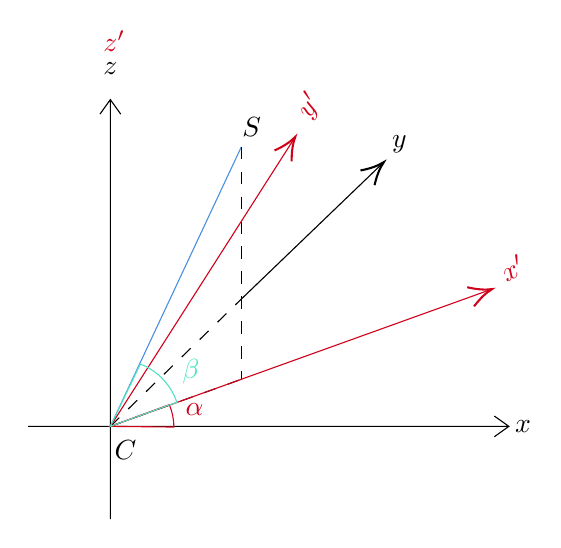
\begin{tikzpicture}[x=0.75pt,y=0.75pt,yscale=-1,xscale=1]
				%uncomment if require: \path (0,300); %set diagram left start at 0, and has height of 300

				%Shape: Axis 2D [id:dp5091691727584546] 
				\draw  (158.44,203.67) -- (390,203.67)(198,46.22) -- (198,248.33) (383,198.67) -- (390,203.67) -- (383,208.67) (193,53.22) -- (198,46.22) -- (203,53.22)  ;
				%Straight Lines [id:da778720861641409] 
				\draw [color={rgb, 255:red, 74; green, 144; blue, 226 }  ,draw opacity=1 ]   (198,203.67) -- (261.11,69) ;
				%Straight Lines [id:da46626427135120685] 
				\draw  [dash pattern={on 4.5pt off 4.5pt}]  (261.11,69) -- (261.11,181) ;
				%Straight Lines [id:da9233448935689583] 
				\draw  [dash pattern={on 4.5pt off 4.5pt}]  (198,203.67) -- (261.11,181) ;
				%Straight Lines [id:da7615405739221883] 
				\draw  [dash pattern={on 4.5pt off 4.5pt}]  (198,203.67) -- (261.11,142.33) ;
				%Straight Lines [id:da03503419757920212] 
				\draw    (261.11,142.33) -- (328.34,77.72) ;
				\draw [shift={(329.78,76.33)}, rotate = 136.13] [color={rgb, 255:red, 0; green, 0; blue, 0 }  ][line width=0.75]    (10.93,-4.9) .. controls (6.95,-2.3) and (3.31,-0.67) .. (0,0) .. controls (3.31,0.67) and (6.95,2.3) .. (10.93,4.9)   ;
				%Straight Lines [id:da5434987803360021] 
				\draw [color={rgb, 255:red, 208; green, 2; blue, 27 }  ,draw opacity=1 ]   (198,203.67) -- (380.01,138.21) ;
				\draw [shift={(381.89,137.53)}, rotate = 160.22] [color={rgb, 255:red, 208; green, 2; blue, 27 }  ,draw opacity=1 ][line width=0.75]    (10.93,-4.9) .. controls (6.95,-2.3) and (3.31,-0.67) .. (0,0) .. controls (3.31,0.67) and (6.95,2.3) .. (10.93,4.9)   ;
				%Shape: Arc [id:dp6588648947058657] 
				\draw  [draw opacity=0] (226.43,193.22) .. controls (227.83,196.61) and (228.6,200.25) .. (228.62,203.98) -- (198,203.67) -- cycle ; \draw  [color={rgb, 255:red, 208; green, 2; blue, 27 }  ,draw opacity=1 ] (226.43,193.22) .. controls (227.83,196.61) and (228.6,200.25) .. (228.62,203.98) -- (198,203.67) -- cycle ;
				%Straight Lines [id:da9325004445855831] 
				\draw [color={rgb, 255:red, 208; green, 2; blue, 27 }  ,draw opacity=1 ]   (198,203.67) -- (286.03,65.85) ;
				\draw [shift={(287.11,64.17)}, rotate = 122.57] [color={rgb, 255:red, 208; green, 2; blue, 27 }  ,draw opacity=1 ][line width=0.75]    (10.93,-4.9) .. controls (6.95,-2.3) and (3.31,-0.67) .. (0,0) .. controls (3.31,0.67) and (6.95,2.3) .. (10.93,4.9)   ;
				%Shape: Arc [id:dp8537237269609406] 
				\draw  [draw opacity=0] (212.48,173.6) .. controls (218.63,176.06) and (223.95,180.41) .. (227.47,186.41) .. controls (228.53,188.23) and (229.38,190.11) .. (230.03,192.04) -- (198,203.67) -- cycle ; \draw  [color={rgb, 255:red, 80; green, 227; blue, 194 }  ,draw opacity=1 ] (212.48,173.6) .. controls (218.63,176.06) and (223.95,180.41) .. (227.47,186.41) .. controls (228.53,188.23) and (229.38,190.11) .. (230.03,192.04) -- (198,203.67) -- cycle ;

				% Text Node
				\draw (198.8,209.47) node [anchor=north west][inner sep=0.75pt]    {$C$};
				% Text Node
				\draw (391.73,199.38) node [anchor=north west][inner sep=0.75pt]    {$x$};
				% Text Node
				\draw (332.53,62.18) node [anchor=north west][inner sep=0.75pt]    {$y$};
				% Text Node
				\draw (193.33,26.98) node [anchor=north west][inner sep=0.75pt]    {$z$};
				% Text Node
				\draw (260.37,53.75) node [anchor=north west][inner sep=0.75pt]    {$S$};
				% Text Node
				\draw (283.87,49.92) node [anchor=north west][inner sep=0.75pt]  [rotate=-306.28]  {$\textcolor[rgb]{0.82,0.01,0.11}{y^{\prime }}$};
				% Text Node
				\draw (233,191.51) node [anchor=north west][inner sep=0.75pt]  [color={rgb, 255:red, 208; green, 2; blue, 27 }  ,opacity=1 ]  {$\alpha $};
				% Text Node
				\draw (193.33,11.84) node [anchor=north west][inner sep=0.75pt]  [color={rgb, 255:red, 208; green, 2; blue, 27 }  ,opacity=1 ]  {$z^{\prime }$};
				% Text Node
				\draw (382.86,125) node [anchor=north west][inner sep=0.75pt]  [rotate=-333.74]  {$\textcolor[rgb]{0.82,0.01,0.11}{x^{\prime }}$};
				% Text Node
				\draw (231.5,169.9) node [anchor=north west][inner sep=0.75pt]    {$\textcolor[rgb]{0.31,0.89,0.76}{\beta }$};


		\end{tikzpicture}
		\caption{绕$z$轴旋转后的坐标系}
		\label{round:system3}
\end{figure}
\noindent 以$SC$为$z$轴的坐标系,首先需要将原始坐标系绕$z$轴逆时针旋转$\alpha$角(如\cref{round:system3}),使得旋转后的坐标轴$x^{\prime}$与直线$SC$在平面$xOy$上的投影重合;由\cref{round:system3}中直线$SC$与$x^{\prime}$轴的夹角$\beta$(图中以青色标出),再将坐标系绕$y^{\prime}$逆时针旋转$(90^{\circ}-\beta)$角即可让坐标系的$z$轴与直线$SC$重合,从而得到以$SC$为$z$轴的坐标系。\par
根据模型准备中对矩阵旋转的推导,第一次将坐标系绕$z$轴逆时针旋转$\alpha$角对应的旋转矩阵为
\[  R_z = \left(
				\begin{array}{ccc}
						\rm{cos}\alpha&\rm{sin}\alpha&0\\
						-\rm{sin}\alpha&\rm{cos}\alpha&0\\
						0&0&1
				\end{array}
		\right)
\]\par
第二次将坐标系绕$y$轴逆时针旋转$(90^{\circ}-\beta)$角对应的旋转矩阵为
\[
		R_y = 
		\left(
				\begin{array}{ccc}
						\rm{cos}(90^{\circ}-\beta)&0&-\rm{sin}(90^{\circ}-\beta)\\
						0&1&0\\
						\rm{sin}((90^{\circ}-\beta))&0&\rm{cos}(90^{\circ}-\beta)
				\end{array}
		\right)
\]

从而,将原始坐标系旋转到以$SC$为$z$轴的坐标系对应的旋转矩阵为


\begin{equation}
		M = R_y R_z = \left(
				\begin{array}{ccc}
						\rm{cos}(90^{\circ}-\beta)&0&-\rm{sin}(90^{\circ}-\beta)\\
						0&1&0\\
						\rm{sin}((90^{\circ}-\beta))&0&\rm{cos}(90^{\circ}-\beta)
				\end{array}
		\right)
		\left(
				\begin{array}{ccc}
						\rm{cos}\alpha&\rm{sin}\alpha&0\\
						-\rm{sin}\alpha&\rm{cos}\alpha&0\\
						0&0&1
				\end{array}
		\right)
\end{equation}

3)基于坐标系旋转变换的理想抛物面计算\par 

把2)中得到的旋转矩阵作用在\texttt{附录1.csv}给出的主索节点坐标上,即得主索节点在以$SC$为$z$轴的坐标系下的新坐标,再根据模型准备中的结论,$300$米口径的旋转抛物面不会超出主动反射面的边界,因此问题2经旋转变换后可转化为问题1的情景。\par
将旋转矩阵作用后的所有主索节点坐标代入问题1的代码中进行求解,可以得到在以$SC$为$z$轴的坐标系下的理想抛物面方程为$z=0.00178(x^2+y^2)-300.89$,根据理想抛物面方程,新坐标系下理想抛物面的顶点坐标为$(0,0,-300.89)$。与问题1中的做法相同,可以通过求直线与抛物面交点来得到新坐标系下反射面$300$米口径内主索节点调节后的坐标,并根据距离公式得到促动器的伸缩量。\par 
由于求得的理想抛物面顶点坐标和反射面$300$米口径内主索节点调节后的坐标都是基于以$SC$为$z$轴的坐标系,还要将这些坐标通过{\bf{逆向旋转}}变换回原始坐标系下的坐标。逆向旋转变换对应的旋转变换矩阵为$M$的逆矩阵,即
\[
		M^{-1}=\left(\left(
						\begin{array}{ccc}
								\rm{cos}(90^{\circ}-\beta)&0&-\rm{sin}(90^{\circ}-\beta)\\
								0&1&0\\
								\rm{sin}((90^{\circ}-\beta))&0&\rm{cos}(90^{\circ}-\beta)
						\end{array}
				\right)
				\left(
						\begin{array}{ccc}
								\rm{cos}\alpha&\rm{sin}\alpha&0\\
								-\rm{sin}\alpha&\rm{cos}\alpha&0\\
								0&0&1
						\end{array}
\right)\right)^{-1}\]

\begin{equation}
		=
		\left(
				\begin{array}{ccc}
						\rm{cos}\alpha&\rm{sin}\alpha&0\\
						-\rm{sin}\alpha&\rm{cos}\alpha&0\\
						0&0&1
				\end{array}
		\right)^{-1}
		\left(
				\begin{array}{ccc}
						\rm{cos}(90^{\circ}-\beta)&0&-\rm{sin}(90^{\circ}-\beta)\\
						0&1&0\\
						\rm{sin}((90^{\circ}-\beta))&0&\rm{cos}(90^{\circ}-\beta)
				\end{array}
		\right)^{-1}
\end{equation}
\par
将矩阵$M^{-1}$作用在上述坐标上即可得到原始坐标系下的理想抛物面顶点坐标和原始坐标系下反射面$300$米口径内主索节点调节后的坐标,以及主索节点$D_{27}$的新的坐标$(-49.3997,-36.9491,-294.4974)$一并按要求存放在\texttt{附件4.xlsx}。\\



\subsection{问题3的模型建立与求解}
问题3是在问题2的条件下求取馈源舱的接收比,并和基准反射球面的接收比进行比较。考虑到落入每个反射面板上的入射光线的量不一致,且反射之后在馈源舱所属平面内的投影三角形与$P$上的中心圆盘的公共面积较难求取,本文采用\textbf{蒙特卡罗模拟方法},在工作态范围内生成竖直向下的入射光线,经反射后观察其最终是否打在中心圆盘上,用圆盘接收到的次数比去实验总次数即得接收比。\par
本问题的研究都基于问题2建立的以$SC$为$z$轴的空间直角坐标系。

\subsubsection{数据预处理}
问题2求得在以$SC$为$z$轴的空间直角坐标系下反射面$300$米口径内主索节点调节后的坐标后,经过旋转矩阵$M^{-1}$的作用,最后获得各点在原始坐标系下反射面$300$米口径内主索节点调节后的坐标。问题3则对上述过程进行改变,获得以$SC$为$z$轴的空间直角坐标系下反射面$300$米口径内主索节点调节后的坐标后,不再用$M^{-1}$作用于各点,直接存放在\texttt{success.csv}待使用。
\newpage
对于\texttt{附件3.csv}中给定的$4300$块反射面板对应的主索节点编号,分别在\texttt{附件1.csv}、\texttt{success.csv}中找到三角形的三个顶点坐标。把每个三角反射面的三个顶点
$A$、$B$、$C$以及与$z$轴正向所成角小于$\frac{\pi}{2}$的法向量$\overrightarrow{n}:(x_1,y_1,z_1), z_1>0$记录在一个三角形字典中。其中用\texttt{附件1.csv}求得的是基准球面的接收比,\texttt{success.csv}则是问题2条件下的接收比。
\subsubsection{利用蒙特卡罗模拟方法生成随机点}
设置蒙特卡罗次数为$1 \times 10^6$。在工作态$300m$口径$x^2 + y^2 \leq r^2$范围内随机生成$x$坐标与$y$坐标,获得入射光出射点$N(x,y,0)$。入射光线从$N$点出发竖直向下,必与一三角形反射面交于反射点$N^{\prime}(x,y,z)$。须确定对应哪一个三角形,才能求得反射光线。
\subsubsection{确定入射光线对应的反射面板和入射点坐标}
根据以$z$轴为对称轴的抛物面的性质,抛物面中所有的三角形反射面板投影到$xOy$平面都是紧密无缝且不重叠的,因此通过二维随机点$P(x,y)$对应的投影后的三角形面板$S_{\Delta}^{\prime}$,可以确定它原本的三角形$S_{\Delta}$,这是一种单射的关系,找到的三角形必唯一。本文通过遍历三角形字典,每次都把三个顶点$A$、$B$、$C$投影到$xOy$平面内获得$A^{\prime}$、$B^{\prime}$、$C^{\prime}$,如\cref{vec}所示用\textbf{向量法}对$P$进行判断。

\begin{figure}[H]
		\centering

		\tikzset{every picture/.style={line width=0.75pt}} %set default line width to 0.75pt        

		\begin{tikzpicture}[x=0.75pt,y=0.75pt,yscale=-1,xscale=1]
				%uncomment if require: \path (0,300); %set diagram left start at 0, and has height of 300

				%Shape: Triangle [id:dp4483629739009378] 
				\draw   (232.67,56) -- (274.33,237.83) -- (73.67,237.83) -- cycle ;
				%Straight Lines [id:da9220598364739967] 
				\draw    (73.67,237.83) -- (200.84,180.65) ;
				\draw [shift={(202.67,179.83)}, rotate = 155.79] [color={rgb, 255:red, 0; green, 0; blue, 0 }  ][line width=0.75]    (13.12,-3.95) .. controls (8.34,-1.68) and (3.97,-0.36) .. (0,0) .. controls (3.97,0.36) and (8.34,1.68) .. (13.12,3.95)   ;
				%Straight Lines [id:da5291059251269696] 
				\draw    (73.67,237.83) -- (231.35,57.51) ;
				\draw [shift={(232.67,56)}, rotate = 131.17] [color={rgb, 255:red, 0; green, 0; blue, 0 }  ][line width=0.75]    (10.93,-4.9) .. controls (6.95,-2.3) and (3.31,-0.67) .. (0,0) .. controls (3.31,0.67) and (6.95,2.3) .. (10.93,4.9)   ;
				%Straight Lines [id:da031015167529194088] 
				\draw    (73.67,237.83) -- (272.33,237.83) ;
				\draw [shift={(274.33,237.83)}, rotate = 180] [color={rgb, 255:red, 0; green, 0; blue, 0 }  ][line width=0.75]    (10.93,-4.9) .. controls (6.95,-2.3) and (3.31,-0.67) .. (0,0) .. controls (3.31,0.67) and (6.95,2.3) .. (10.93,4.9)   ;
				%Straight Lines [id:da24050436649535412] 
				\draw  [dash pattern={on 4.5pt off 4.5pt}]  (123.47,180.63) -- (202.67,179.83) ;
				%Straight Lines [id:da30914064217236525] 
				\draw  [dash pattern={on 4.5pt off 4.5pt}]  (202.67,179.83) -- (146.67,237.83) ;

				% Text Node
				\draw (52,234.4) node [anchor=north west][inner sep=0.75pt]    {$A^{\prime}$};
				% Text Node
				\draw (276.33,241.23) node [anchor=north west][inner sep=0.75pt]    {$B^{\prime}$};
				% Text Node
				\draw (227,33.4) node [anchor=north west][inner sep=0.75pt]    {$C^{\prime}$};
				% Text Node
				\draw (211,169.4) node [anchor=north west][inner sep=0.75pt]    {$P$};
				% Text Node
				\draw (156,251.4) node [anchor=north west][inner sep=0.75pt]    {$\vec{u}$};
				% Text Node
				\draw (129,132.4) node [anchor=north west][inner sep=0.75pt]    {$\vec{v}$};


		\end{tikzpicture}
		\caption{用向量法判定点$P$是否在$\Delta A^{\prime}B^{\prime}C^{\prime}$中}
		\label{vec}
\end{figure}

根据平面中的任意向量可以由两不共线非零向量的线性组合表示,在$\Delta A^{\prime}B^{\prime}C^{\prime}$中,有
$\overrightarrow{A^{\prime}P} = \mu \overrightarrow{A^{\prime}C^{\prime}} + \lambda \overrightarrow{A^{\prime}B^{\prime}}$。那么$P$在$\Delta A^{\prime}B^{\prime}C^{\prime}$中的充分必要条件是:$\mu > 0$
,$\lambda > 0$且$\mu + \lambda < 1$。根据上述方法对每次取得的三角形进行判断,当满足以上所有条件时,即找到了三维随机点$N$竖直向下发出入射光线所对应的反射面三角形$S_{\Delta \rm{in}}$,停止遍历。
\newpage
在先前创建的三角形字典中获取$S_{\Delta \rm{in}}$的其中一个顶点$A(x_A,y_A,z_A)$及其法向量$\overrightarrow{n}(x_1,y_1,z_1)$,得出$S_{\Delta \rm{in}}$所在平面$S_{ABC}$的方程:
\begin{equation}
		S_{ABC}: \quad x_1(x-x_A)+y_1(y-y_A)+z_1(z-z_A) = 0
\end{equation}\par 
由于入射光线竖直向下,将$N(x,y,0)$代入即可得出反射点$N^{\prime}(x,y,z)$,其中
\begin{equation}
		z =  \frac{x_1(x_A-x)+y_1(y_A-y)}{z_1} + z_A
\end{equation}
\subsubsection{利用几何关系判断反射光线是否打在馈源舱内}
\begin{figure}[H]
		\centering






		\tikzset{every picture/.style={line width=0.75pt}} %set default line width to 0.75pt        

		\begin{tikzpicture}[x=0.75pt,y=0.75pt,yscale=-1,xscale=1]
				%uncomment if require: \path (0,405); %set diagram left start at 0, and has height of 405

				%Straight Lines [id:da0197186749099012] 
				\draw    (93.56,75.11) -- (93.67,269) ;
				\draw [shift={(93.67,271)}, rotate = 269.97] [color={rgb, 255:red, 0; green, 0; blue, 0 }  ][line width=0.75]    (10.93,-3.29) .. controls (6.95,-1.4) and (3.31,-0.3) .. (0,0) .. controls (3.31,0.3) and (6.95,1.4) .. (10.93,3.29)   ;
				%Straight Lines [id:da8520942591705003] 
				\draw  [dash pattern={on 4.5pt off 4.5pt}]  (183.56,130.89) -- (93.67,271) ;
				%Straight Lines [id:da14289492093965794] 
				\draw    (93.67,271) -- (404.04,130.86) ;
				\draw [shift={(405.87,130.04)}, rotate = 155.7] [color={rgb, 255:red, 0; green, 0; blue, 0 }  ][line width=0.75]    (10.93,-3.29) .. controls (6.95,-1.4) and (3.31,-0.3) .. (0,0) .. controls (3.31,0.3) and (6.95,1.4) .. (10.93,3.29)   ;
				%Straight Lines [id:da3572030555623502] 
				\draw    (93.47,130.44) -- (405.87,130.04) ;
				%Straight Lines [id:da6503440844985282] 
				\draw    (26.67,231.99) -- (187.67,326.99) ;
				%Shape: Arc [id:dp684421240995355] 
				\draw  [draw opacity=0] (93.81,242.09) .. controls (99.28,242.32) and (104.81,244.05) .. (109.73,247.4) .. controls (114.3,250.51) and (117.77,254.62) .. (120.02,259.21) -- (93.67,271) -- cycle ; \draw   (93.81,242.09) .. controls (99.28,242.32) and (104.81,244.05) .. (109.73,247.4) .. controls (114.3,250.51) and (117.77,254.62) .. (120.02,259.21) -- (93.67,271) -- cycle ;
				%Straight Lines [id:da5733104813392218] 
				\draw    (93.67,271) -- (108.86,247.05) ;
				%Straight Lines [id:da17738233422214256] 
				\draw    (93.67,271) -- (146.42,188.37) ;
				\draw [shift={(147.5,186.68)}, rotate = 122.56] [color={rgb, 255:red, 0; green, 0; blue, 0 }  ][line width=0.75]    (10.93,-4.9) .. controls (6.95,-2.3) and (3.31,-0.67) .. (0,0) .. controls (3.31,0.67) and (6.95,2.3) .. (10.93,4.9)   ;

				% Text Node
				\draw (103.49,224.3) node [anchor=north west][inner sep=0.75pt]  [rotate=-20.2]  {$\theta $};
				% Text Node
				\draw (122.84,233.46) node [anchor=north west][inner sep=0.75pt]  [rotate=-28.44]  {$\theta $};
				% Text Node
				\draw (152.67,185.4) node [anchor=north west][inner sep=0.75pt]    {$\vec{n}$};
				% Text Node
				\draw (75.33,62.07) node [anchor=north west][inner sep=0.75pt]    {$N$};
				% Text Node
				\draw (83.27,277.09) node [anchor=north west][inner sep=0.75pt]    {$N^{\prime }$};
				% Text Node
				\draw (407.87,133.44) node [anchor=north west][inner sep=0.75pt]    {$N^{\prime \prime }$};
				% Text Node
				\draw (73,123.4) node [anchor=north west][inner sep=0.75pt]    {$T$};


		\end{tikzpicture}
		\caption{入射光线的反射图像}
		\label{reflect}
\end{figure}


根据5.3.3,点$N^{\prime}$的坐标为$(x,y,z)$,法向量$\vec{n}=(x_1,y_1,z_1)$,因此由\cref{reflect}的几何关系可得
\begin{equation}
		{\rm{cos}} \theta = \frac{(x_1,y_1,z_1)\cdot(0,0,1)}{\sqrt{{x_1}^2+{y_1}^2+{z_1}^2}}=\frac{z_1}{\sqrt{{x_1}^2+{y_1}^2+{z_1}^2}}
		\label{theta}
\end{equation}\par
直线$TN^{\prime \prime}$位于馈源舱所在平面上,故有
\begin{equation}
		|TN^{\prime}| = |z| - |CP|
		\label{TN'}
\end{equation}\par
又由于
\begin{equation}
		|TN^{{\prime}{\prime}}| = |TN^{\prime}| \cdot \rm{tan}2\theta
		\label{TN''}
\end{equation}\par
将\cref{theta}\cref{TN'}代入\cref{TN''}中可得
\begin{equation}
		|TN^{{\prime}{\prime}}| = (|z| - |CP|)\cdot \frac{2z_1\sqrt{{x_1}^2+{y_1}^2}}{{z_1}^2-{x_1}^2-{y_1}^2}
\end{equation}
\newpage
在馈源舱所处的二维$xOy$平面内,对$TN^{{\prime}{\prime}}$算出在$x$与$y$方向上的分量
\begin{equation}
		\overrightarrow{{TN^{{\prime}{\prime}}}}=(|{TN^{{\prime}{\prime}}}|\frac{x_1}{\sqrt{{x_1}^2+{y_1}^2}},|{TN^{{\prime}{\prime}}}|\frac{y_1}{\sqrt{{x_1}^2+{y_1}^2}})
		\label{vec_show}
\end{equation}\par 
而点$T$的坐标为$(x_1,y_1)$,故点$N^{\prime \prime}$的坐标为
\begin{equation}	
		\begin{aligned}
				\left(x_{N^{\prime \prime}},y_{N^{\prime \prime}}\right) &= \left(x_1+|{TN^{{\prime}{\prime}}}|\frac{x_1}{\sqrt{{x_1}^2+{y_1}^2}},\quad y_1+|{TN^{{\prime}{\prime}}}|\frac{y_1}{\sqrt{{x_1}^2+{y_1}^2}}\right)\\
				\\
																		 &=\left(x_1+\frac{2(|z| - |CP|)x_1 z_1}{{z_1}^2-{x_1}^2-{y_1}^2},\quad 
																		 y_1+\frac{2(|z| - |CP|)y_1 z_1}{{z_1}^2-{x_1}^2-{y_1}^2}\right)
		\end{aligned}
		\label{N''loc}	
\end{equation}\par 

由于馈源舱的接受范围为$x^2+y^2 \leq p^2$($p$为馈源舱的半径,大小为0.5米),因此只有满足${x_{N^{\prime \prime}}}^2+{y_{N^{\prime \prime}}}^2\leq p^2$的入射光线才能成为有效的入射光线,代入\cref{N''loc}中的$\left(x_{N^{\prime \prime}},y_{N^{\prime \prime}}\right)$即可得解。\\

\subsubsection{问题3的结果分析}
\begin{table}[H]   
		\begin{center}
				\begin{tabular}{ccc}
						\hline
						\makebox[0.2\textwidth][c]{ } &
						\makebox[0.35\textwidth][c]{基准球面接收比} &
						\makebox[0.35\textwidth][c]{调整面板后接收比} \\ \hline
						$1$   &   $0.7695\%$    &   $1.1572\%$\\
						$2$   &   $0.7518\%$    &   $1.1307\%$\\
						$3$   &   $0.7716\%$    &   $1.1268\%$\\
						$4$   &   $0.7647\%$    &   $1.1274\%$\\
						$5$   &   $0.7600\%$    &   $1.1345\%$\\ \hline
						平均值 &   $0.7635\%$    &   $1.1353\%$\\ \hline
				\end{tabular}
		\end{center}
		\caption{五次蒙特卡罗模拟结果及平均值}
		\label{fiveavg}
\end{table}
经过以上方法计算,获得的数据存放于\cref{fiveavg}。
最终结论为:基于问题2的反射面调节方案,所得的馈源舱接收比为$\bm{1.1353\%}$,
基准反射球面的接收比为$\bm{0.7625\%}$,调节之后的接收比提升率为$\bm{48.69\%}$,提升效果显著。

\newpage
\section{模型评价与推广}
\subsection{模型优点}
1. 在对$b$进行变步长搜索的过程中,通过研究抛物面上的点到$C$点距离的单调性,只需对特定位置的三个点的伸缩量进行检查,避开了对所有主索节点伸缩量的依次检查,极大减小了算法的时间复杂度。\par 
2. 问题3采用蒙特卡罗模拟的方法,通过在馈源舱范围内生成随机点,来模拟光线的入射,一方面省却了繁复的数学演算过程,另一方面降低了问题的建模难度,不必考虑不同三角形反射面在反射后于馈源舱平面处的投影三角形与中心圆盘的重合面积的问题。
\subsection{模型缺点}
1. 在寻找理想抛物面时,没有根据要求的"相邻主索节点坐标之间距离变化幅度不超过$0.07\%$”将“相邻主索节点坐标之间距离变化尽可能小”作为优化条件之一。\par 
2. 在寻找理想抛物面时,仅从几何的角度考虑问题,而没有从力学角度考虑各主索节点伸缩时的受力情况,从减小受力的角度对模型进行进一步优化。
\subsection{模型的改进和推广}
1. 可以对主索节点的伸缩过程进行应力分析,从而找到对索网结构破坏最小的伸缩方案。\par 
2. 由于该模型可以给出不同情况下馈源舱有效区域的接收比,因此基于计算问题1、问题2的模型可以进一步对每一块三角形做单独调整,使其顶点不必位于理想抛物面内,以使得馈源舱有效区域可获得最大接收比。
\newpage
\begin{thebibliography}{9} % 参考文献
		\bibitem{bib:one}
		南仁东.
		\newblock 500m球反射面射电望远镜FAST\allowbreak [J].
		\newblock 中国科学G辑:物理学、力学、天文学,2005.
		\bibitem{bib:two}
		钱宏亮.
		\newblock FAST主动反射面支承结构理论与试验研究\allowbreak [D].
		\newblock 哈尔滨工业大学,2007.
\end{thebibliography}
\begin{appendices}  
		\begin{lstlisting}[language={python}]  
		# 问题一核心代码

		import pandas as pd
		import numpy as np

		data = pd.read_csv('data1.csv', usecols=range(1, 4),
		encoding="gbk", dtype=float)

		# 新建一个存放b所对应的促动器变化值总和的字典
		b_dict = {}

		# b在[-301, -299.8]的范围之间变动,把0.001作为变化步长进行遍历:
		# -301, -299.8, 0.01
		# -301, -299.8, 0.001
		# -300.95, -300.85, 0.0001
		for b in np.arange(-301, -299.8, 0.001):

		# 针对第一问的条件,由 f + CP = |b| 可得a关于b的函数关系
		a = 1/(4*(-b - 0.534*300.4))

		"""
		在yOz平面中研究促动器伸缩量,取z = a*y^2 + b平面进行研究
		通过观察,发现理想抛物面上的点到原点C的距离d满足从顶点A0'到z = -1/2a的点先变小,
		再到工作态抛物面边界的点(满足sqrt(x^2 + y^2) = 150)又变大的单调性关系
		因此确定筛选条件:1. sqrt(z^2 + y^2) - R >= -0.6   ,  z = -1/2a
		2. sqrt(z^2 + y^2) - R <= +0.6   ,  y = 150
		"""
		if (-b/a - 1/(4*a**2))**0.5 - 300.4 < -0.6 or (150**2 + (a*150**2+b)**2)**0.5 - 300.4 > 0.6:
		continue
		else:
		b_dict[b] = 0
		for row in data.iloc:
		x0 = row[0]
		y0 = row[1]
		z0 = row[2]
		if x0**2 + y0**2 <= 22591:   # 根据极端情况  筛掉无用的点
		# 计算新的主索节点的纵坐标z1

		"""
		先转化为求平面上的交点的问题
		联立:1. z = a*y^2 + b
		2. z = z0/sqrt(x0^2 + y0^2) * y
		解得关于z的一元二次方程 Az^2 + Bz + C = 0
		"""
		A = a*((x0*x0+y0*y0)/(z0*z0))
		B = -1
		C = b
		if A != 0:
		# 所求的点在xOy平面以下,满足z<0,故取较小的z1
		z1 = (-B-(B*B-4*A*C)**0.5)/(2*A)
		y1 = (z1/z0) * y0
		x1 = (z1/z0) * x0
		# 根据相似关系 d = R - R(z1/z0)
		d = 300.4*(1-z1/z0)
		# 仅取工作态范围内的点
		if x1 ** 2 + y1 ** 2 <= 22500:
		b_dict[b] += abs(d)
		else:
		# 最终加上顶点的变化量(因为顶点的xy坐标均为0,需要单独计算)
		b_dict[b] += abs(300.4 + b)

		# final_b为最终确定的最优参数
		final_b = 0
		min_sum = np.inf
		# 遍历字典求得最小变化量所对应的b
		for (key, value) in b_dict.items():
		if value < min_sum:
		min_sum = value
		final_b = key
		final_a = 1/(4*(-final_b - 0.534*300.4))

		print(f"z = {round(final_a,7)}(x^2+y^2)+{round(final_b,4)}")

		\end{lstlisting}  % 此处粘贴python代码
		\begin{lstlisting}[language={python}]  
		# 问题2核心代码
		import pandas as pd
		import numpy as np
		import openpyxl as op

		alpha = np.deg2rad(36.795)
		gamma = np.deg2rad(90 - 78.169)




		# 计算旋转矩阵
		Rz = np.array([[np.cos(alpha),  np.sin(alpha), 0],
		[-np.sin(alpha), np.cos(alpha), 0],
		[0,              0,             1]])

		Ry = np.array([[np.cos(gamma), 0, -np.sin(gamma)],
		[0,             1,              0],
		[np.sin(gamma), 0,  np.cos(gamma)]])

		R = Ry @ Rz
		R_inv = np.linalg.inv(R)

		data = pd.read_csv('data1.csv', usecols=range(0, 4), encoding="gbk")

		a_dict = {}

		# i表示数据表中的行索引
		i = 0

		for row in data.iloc:
		x0 = row[1]
		y0 = row[2]
		z0 = row[3]
		# 求出每点在新坐标系下的坐标,并保存至a_dict
		A_0 = R @ [[x0], [y0], [z0]]
		a_dict[i] = A_0
		i = i + 1

		# 新建一个存放b所对应的促动器变化值总和的字典
		b_dict = {}

		# b在[-301, -299.8]的范围之间变动,把0.001作为变化步长进行遍历:
		for b in np.arange(-301, -299.8, 0.001):

		# 针对第一问的条件,由 f + CP = |b| 可得a关于b的一次函数关系
		a = 1 / (4 * (- b - 0.534 * 300.4))

		"""
		在yOz平面中研究促动器伸缩量,取z = a * y ^ 2 + b平面进行研究
		通过观察,发现理想抛物面上的点到原点C的距离d满足从顶点A0'到z = -1/2a的点先变小,
		再到工作态抛物面边界的点(满足sqrt(x^2 + y^2) = 150)又变大的单调性关系
		因此确定筛选条件:1. sqrt(z^2 + y^2) - R >= -0.6   ,  z = -1/2a
		2. sqrt(z^2 + y^2) - R <= +0.6   ,  y = 150
		"""
		if (-b/a - 1/(4*a**2))**0.5 - 300.4 < -0.6 or (150**2 + (a*150**2+b)**2)**0.5 - 300.4 > 0.6:
		continue
		else:
		b_dict[b] = 0
		for j in range(0, i):
		x0 = a_dict[j][0][0]
		y0 = a_dict[j][1][0]
		z0 = a_dict[j][2][0]
		# 仅取工作态范围内的点  计算新的主索节点的纵坐标z1
		if x0**2+y0**2 <= 22591:
		"""
		先转化为求平面上的交点的问题
		联立:1. z = a*y^2 + b
		2. z = z0/sqrt(x0^2 + y0^2) * y
		解得关于z的一元二次方程 Az^2 + Bz + C = 0
		"""
		A = a*((x0*x0+y0*y0)/(z0*z0))
		B = -1
		C = b
		if A != 0:
		# 所求的点在xOy平面以下,满足z<0,故取较小的z1
		z1 = (-B-(B*B-4*A*C)**0.5)/(2*A)
		x1 = (z1/z0) * x0
		y1 = (z1/z0) * y0
		# 根据相似关系 d = R - R(z1/z0)
		d = 300.4*(1-z1/z0)

		if x1 ** 2 + y1 ** 2 <= 22500:
		b_dict[b] += abs(d)
		else:
		# 最终加上顶点的变化量(因为顶点的xy坐标均为0,需要单独计算)
		b_dict[b] += abs(300.4 + b)

		# final_b为最终确定的最优参数
		final_b = 0
		min_sum = np.inf
		# 遍历字典求得最小变化量所对应的b
		for (key, value) in b_dict.items():
		if value < min_sum:
		min_sum = value
		final_b = key
		final_a = 1/(4*(-final_b - 0.534*300.4))

		print(f"z = {round(final_a,6)}(x^2+y^2){round(final_b,3)}")


		# 写.xlsx文件前的准备工作
		workbook = op.Workbook()
		worksheet1 = workbook.active
		worksheet1.title = "调整后主索节点编号及坐标"
		worksheet2 = workbook.create_sheet(title="促动器顶端伸缩量")
		worksheet3 = workbook.create_sheet(title="理想抛物面顶点坐标")
		dat1 = [["节点编号", "X坐标(米)", "Y坐标(米)", "Z坐标(米)"]]
		dat2 = [["对应主索节点编号", "伸缩量(米)"]]
		A_3 = R_inv@[[0], [0], [-300.89]]
		dat3 = [["X坐标(米)", "Y坐标(米)", "Z坐标(米)"]]
		dat3.append([A_3[0][0], A_3[1][0], A_3[2][0]])

		'''
		新坐标系下点(x0, y0, z0)对应的直线参数方程为x=x0*t, y=y0*t, z=z0*t
		与求得的抛物线z = 0.00178(x^2+y^2)-300.89联立可得一元二次方程:
		(0.00178*(x0**2 + y0**2)) * x^2+ (-z0) * x + (-300.89) = 0
		即可解出交点坐标
		'''
		for j in range(0, i):
		x0 = a_dict[j][0][0]
		y0 = a_dict[j][1][0]
		z0 = a_dict[j][2][0]
		# 求解一元二次方程
		D = 0.00178*(x0**2 + y0**2)
		E = -z0
		F = -300.89
		if D != 0:
		t = (-E + (E**2 - 4 * D * F)**0.5)/(2*D)
		x1 = t*x0
		y1 = t*y0
		z1 = t*z0
		if x1**2+y1**2 <= 22500:
		A_1 = R_inv @ [[x1], [y1], [z1]]
		dat1.append([data.iloc[j][0], A_1[0][0], A_1[1][0], A_1[2][0]])
		dat2.append([data.iloc[j][0], (x1**2+y1**2+z1**2)**0.5-300.4])
		else:
		A_1 = R_inv @ [[0], [0], [final_b]]
		dat1.append([data.iloc[j][0], A_1[0][0], A_1[1][0], A_1[2][0]])
		dat2.append([data.iloc[j][0], (x1**2+y1**2+z1**2)**0.5-300.4])

		# 将获得的结果写入result.xlsx文件
		for row in dat1:
		worksheet1.append(row)
		for row in dat2:
		worksheet2.append(row)
		for row in dat3:
		worksheet3.append(row)
		workbook.save(filename="result.xlsx")

		\end{lstlisting}  % 此处粘贴python代码
		\begin{lstlisting}[language={python}]  
		# 问题3核心代码

		import numpy as np
		import pandas as pd
		import random
		import winsound
		alpha = np.deg2rad(36.795)
		gamma = np.deg2rad(90 - 78.169)
		# 计算旋转矩阵
		Rz = np.array([[np.cos(alpha),  np.sin(alpha), 0],
		[-np.sin(alpha), np.cos(alpha), 0],
		[0,              0,             1]])

		Ry = np.array([[np.cos(gamma), 0, -np.sin(gamma)],
		[0,             1,              0],
		[np.sin(gamma), 0,  np.cos(gamma)]])

		R = Ry @ Rz
		position_dict = {}
		position_dict_strict = {}

		# 基准态球面
		data1 = pd.read_csv('data1.csv', usecols=range(0, 4), encoding="gbk")
		# 问题2情况计算
		# data1 = pd.read_csv('success.csv', usecols=range(0, 4), encoding="gbk")
		data3 = pd.read_csv('data3.csv', usecols=range(0, 3), encoding="gbk")


		for row in data1.iloc:
		x0 = row[1]
		y0 = row[2]
		z0 = row[3]
		# 求出每点在新坐标系下的坐标,并保存至a_dict
		A_0 = [[x0], [y0], [z0]]
		# 去掉内层中括号
		A_1 = [A_0[0][0], A_0[1][0], A_0[2][0]]
		# 取处在工作态及附近的点
		if x0**2+y0**2 <= 180**2:
		position_dict[row[0]] = A_1
		if x0**2+y0**2 <= 150**2:
		position_dict_strict[row[0]] = A_1

		triangle_dict = {}
		i = 0
		for row in data3.iloc:
		A = row[0]
		B = row[1]
		C = row[2]

		if (A in position_dict_strict) or (B in position_dict_strict) or (C in position_dict_strict):
		A_position = position_dict[A]
		B_position = position_dict[B]
		C_position = position_dict[C]
		# 求三角形重心
		G = [(A_position[0] + B_position[0] + C_position[0])/3, (A_position[1] + B_position[1] + C_position[1]) /
		3, (A_position[2] + B_position[2] + C_position[2])/3]
		# 求沿z轴正方向的法向量

		VEC_AB = np.array([B_position[0]-A_position[0],
		B_position[1]-A_position[1],
		B_position[2]-A_position[2]])
		VEC_AC = np.array([C_position[0]-A_position[0],
		C_position[1]-A_position[1],
		C_position[2]-A_position[2]])
		n = np.cross(VEC_AB, VEC_AC)
		if (n[2] < 0):
		n = [-n[0], -n[1], -n[2]]
		else:
		n = [n[0], n[1], n[2]]
		# 将A\B\C和法向量存入三角形字典
		triangle_dict[i] = [A_position,B_position,C_position, n]
		i = i + 1

		# 根据蒙特卡罗法,随机生成位于工作态内的坐标(x, y)
		# 记录距离随机点最近的三角形
		triangle_close = []
		righttimes = 0
		wrongtimes = 0
		# 设置蒙特卡洛实验次数
		mc_times = 1000000
		for j in range(0, mc_times):
		print(j)
		dis = np.inf
		x = random.randrange(-150, 150)
		y = random.randrange(-150, 150)

		if ((x**2 + y**2) > 150**2):
		continue
		for num, tri in triangle_dict.items():
		u = x - tri[0][0]
		v = y - tri[0][1]
		m = tri[1][0] - tri[0][0]
		n = tri[1][1] - tri[0][1]
		r = tri[2][0] - tri[0][0]
		s = tri[2][1] - tri[0][1]
		a = (s * u - r * v) / (s * m - r * n)
		b = (n * u - m * v) / (n * r - m * s)
		if(a > 0) and (b > 0) and (a + b < 1):
		triangle_close = tri
		break
		A_close = triangle_close[0]
		n_close = triangle_close[3]
		z = (A_close[0] * n_close[0] + A_close[1] * n_close[1] +
		A_close[2] * n_close[2] - n_close[0]*x - n_close[1]*y)/n_close[2]
		# 计算光线投影在馈源舱平面的坐标

		x1 = n_close[0]
		y1 = n_close[1]
		z1 = n_close[2]
		z_prime = abs(z)-0.534 * 300.4
		x_reflect = x + 2 * x1 * z1*z_prime/(z1*z1-(x1*x1+y1*y1))
		y_reflect = y + 2 * y1 * z1*z_prime/(z1*z1-(x1*x1+y1*y1))


		if (x_reflect**2+y_reflect**2) <= 0.5**2:
		righttimes = righttimes + 1
		else:
		wrongtimes = wrongtimes + 1
		print(righttimes / (righttimes + wrongtimes))

		\end{lstlisting}  % 此处粘贴python代码
\end{appendices}
\end{document}
